\documentclass[../DoAn.tex]{subfiles}
\begin{document}

\section{Thiết kế kiến trúc}
\subsection{Lựa chọn kiến trúc phần mềm}
% Mục này có độ dài từ một đến ba trang. Sinh viên cần lựa chọn kiến trúc phần mềm cho ứng dụng của mình như: kiến trúc ba lớp MVC, MVP, SOA, Microservice, v.v. rồi giải thích sơ bộ về kiến trúc đó (không giải thích chi tiết/dài dòng).
% Sử dụng kiến trúc phần mềm đã chọn ở trên, sinh viên mô tả kiến trúc cụ thể cho ứng dụng của mình. Gợi ý: sinh viên áp dụng lý thuyết chung vào hệ thống/sản phẩm của mình như thế nào, có thay đổi, bổ sung hoặc cải tiến gì không. Ví dụ, thành phần M trong kiến trúc lý thuyết MVC sẽ là những thành phần cụ thể nào (ví dụ: là interface I + class C1 + class C2, v.v.) trong kiến trúc phần mềm của sinh viên.

Trong đồ án này, tôi lựa chọn kiến trúc phần mềm MVC (Model-View-Controller).
Kiến trúc phần mềm theo mô hình MVC là một trong những mô hình phổ biến và được sử dụng rộng rãi trong việc phát triển ứng dụng. Mô hình này giúp tách biệt các thành phần chức năng của ứng dụng thành ba phần riêng biệt, đảm bảo tính dễ dàng trong việc quản lý, bảo trì và mở rộng ứng dụng. Ba thành phần chính của mô hình MVC bao gồm:

\textbf{Model (M)}: Đây là thành phần chịu trách nhiệm quản lý dữ liệu và logic nghiệp vụ của ứng dụng. Model xử lý tất cả các hoạt động liên quan đến dữ liệu như lấy, lưu trữ, cập nhật và xóa dữ liệu. Nó không phụ thuộc vào giao diện người dùng, điều này giúp dữ liệu và logic nghiệp vụ có thể được tái sử dụng và kiểm thử dễ dàng hơn.

\textbf{View (V)}: Thành phần này chịu trách nhiệm hiển thị dữ liệu cho người dùng và nhận các tương tác từ họ. View là giao diện người dùng của ứng dụng, nó có thể là các trang web HTML, các form trong ứng dụng desktop hay các màn hình trong ứng dụng di động. View chỉ nên phụ thuộc vào Model để lấy dữ liệu và không chứa logic nghiệp vụ.

\textbf{Controller (C)}: Đây là thành phần trung gian giữa Model và View. Controller nhận các yêu cầu từ người dùng thông qua View, xử lý các yêu cầu này và tương tác với Model để lấy hoặc cập nhật dữ liệu. Sau đó, Controller quyết định View nào sẽ hiển thị dữ liệu đó cho người dùng. Controller giúp duy trì sự tách biệt giữa Model và View, đảm bảo rằng mỗi thành phần chỉ thực hiện nhiệm vụ của mình.

Thành phần M trong kiến trúc MVC khi được triển khai trong đồ án của tôi bao gồm:

\textbf{Entity}: Là package bao gồm các lớp java đại diện cho các thực thể trong hệ thống. Trong đồ án của tôi đã viết các lớp sau: Address, BaseEntity, Book, BookCategory, CartItem, City, Comment, Complain, Country, Coupon, ConponCondition, Customer, Favorite, Order, OrderItem, OrderStatus, Role, SocialAccount,Token, User.

\textbf{DAO}: DAO(Data Access Object) là nhứng interface kế thừa từ JPARepository dùng để truy xuất cơ sỏ dữ liệu. Trong đồ án của tôi, bao gồm các interface sau: BookCategory, Book, CartItem, City, Comment, Complain, Country, CouponCondition, Coupon, Customer, Favorite, OrderItem, Order, Role, Token, user

\textbf{DTO}: DTO(Data Transfer Object) là các lớp được sử dụng cho việc truyền dữ liệu giữa các hệ thống trong một ứng dụng.Mục đích của DTO trong thiết kế hệ thống bao gồm:


\begin{enumerate}
  \item[(i)] \textbf{Đơn giản hóa việc truyền dữ liệu}: DTO giúp gom nhóm các thuộc tính dữ liệu liên quan thành một đối tượng duy nhất, giúp việc truyền tải dữ liệu trở nên dễ dàng và có tổ chức hơn.
  \item[(ii)] \textbf{Bảo mật dữ liệu}: DTO giúp kiểm soát dữ liệu được truyền đi, chỉ bao gồm các thuộc tính cần thiết và bỏ qua các thông tin nhạy cảm hoặc không cần thiết.
  \item[(iii)] \textbf{Tăng tính linh hoạt}: DTO cung cấp một cách để thay đổi cấu trúc dữ liệu được truyền mà không ảnh hưởng đến các tầng khác của ứng dụng.
\end{enumerate}

Trong đồ án của tôi bao gồm các lớp DTO sau: BookCategory, Book, CartItem, Comment, Complain, Order, OrderItem, Paymentinfo, Purchase, RefreshToken, UpdateUser, User, UserLogin.

\textbf{Responses}: Là nhứng lớp được sử dụng để phản hồi từ server về client. Mục đích của response bao gồm :
\begin{enumerate}
  \item[(i)] \textbf{Đảm bảo tính nhất quán}: các lớp  Responses giúp đảm bảo cấu trúc trả về từ API luôn nhất quán
  \item[(ii)] \textbf{Bảo mật dữ liệu}:Chỉ những thông tin cần thiết mới được đưa vào trong các lớp Responses để trả về client, giúp tăng cường bảo mật.
  \item[(iii)] \textbf{Dễ dàng mở rộng và bảo trì}: khi yêu cầu phản hồi thay đổi, các lớp Responses có thể được cập nhật dễ dàng mà không gây ảnh hưởng đến các phần khác của ứng dụng.
\end{enumerate}

Trong đồ án của tôi bao gồm các lớp Responses sau: Book, CartItem, Comment, Complain, CouponCalculation, Favorite, OrderItem, Order, Purchase, Login, User, Base, ResponseObject, ResponsePageObject, BookList.

\textbf{Service}: Các lớp Service đóng vai trò trung gian giữa tầng Controller và tầng Repository (hoặc tầng dữ liệu), nơi chúng thực hiện các logic nghiệp vụ phức tạp, thao tác và xử lý dữ liệu trước khi gửi đến hoặc nhận từ cơ sở dữ liệu. Vai trò cụ thể của các lớp này bao gồm:

\begin{enumerate}
  \item[(i)] \textbf{Xử lý logic nghiệp vụ }: Các lớp Service chứa logic nghiệp vụ chính của ứng dụng. Chúng thực hiện các thao tác phức tạp liên quan đến dữ liệu và nghiệp vụ mà không để logic này lẫn vào tầng Controller hoặc Repository.
  \item[(ii)] \textbf{Tăng tính tái sử dụng}:Logic nghiệp vụ được cô lập trong các lớp Service có thể được tái sử dụng bởi nhiều Controller hoặc các thành phần khác của ứng dụng.
  \item[(iii)] \textbf{Giảm sự phụ thuộc giữa các tầng}: Service giúp tách biệt các tầng của ứng dụng, đảm bảo rằng tầng Controller không phụ thuộc trực tiếp vào tầng Repository. Điều này giúp tăng tính linh hoạt và dễ dàng bảo trì.
  \item[(iv)] \textbf{Quản lý giao dịch}:  Trong các ứng dụng cần quản lý giao dịch (transaction), Service là nơi thích hợp để thực hiện và quản lý các giao dịch này.
\end{enumerate}

Trong đồ án của tôi, các lớp và các interface Service tương ứng bao gồm: BookRedis, Book, BookCategory, CartItem, Checkout, Comment, Complain, Coupon, Order, OrderItem, Role, Token, User.

Thành phần C trong kiến trúc MVC bao gồm các lớp Controller chịu trách nhiệm trung gian giữa Model và View. Các lớp Controller sẽ nhận yêu càu từ phía client, tương tác với model đê truy xuất hoặc cập nhật dữ liệu và trả lại kết quả về cho bên phía client.

Trong đồ án của tôi, các lớp Controller bao gồm: BookCategory, Book, CartItem, Checkout, Comment, Complain, Coupon, Order, OrderItem, Role, User.

Thành phần V trong mô hình MVC bao gồm toàn bộ hệ thống front-end được viết bằng angularJS.


\subsection{Thiết kế tổng quan}

Trong biểu đồ ở Hình \ref{fig:Fig1} các gói được phân chia theo các tầng và sự phụ thuộc giữa các gói được biểu thị bằng các mũi tên đứt nét, nhằm thể hiện rằng một gói này phụ thuộc vào gói khác. Dưới đây là giải thích sơ lược về mục đích và nhiệm vụ của từng package:

\textbf{controller}:
\begin{enumerate}
    \item [(i)]\textbf{Mục đích}: Chứa các lớp điều khiển, chịu trách nhiệm xử lý và phản hồi các yêu cầu từ người dùng và điều hướng chúng đến các dịch vụ tương ứng.
    \item [(ii)]\textbf{Phụ thuộc}: Phụ thuộc vào utils, component, config, dto, service, exceptions và responses.
\end{enumerate}

\textbf{config}:
\begin{enumerate}
    \item [(i)]\textbf{Mục đích}: Chứa các lớp cấu hình của ứng dụng.
    \item [(ii)]\textbf{Phụ thuộc}: Phụ thuộc vào filters.
\end{enumerate}

\textbf{service}:
\begin{enumerate}
    \item [(i)]\textbf{Mục đích}: Chứa các lớp dịch vụ, nơi thực hiện các logic nghiệp vụ chính của ứng dụng.
    \item [(ii)]\textbf{Phụ thuộc}: Phụ thuộc vào component, dto, dao và exceptions/
\end{enumerate}

\textbf{responses}:
\begin{enumerate}
    \item [(i)]\textbf{Mục đích}: Chứa các lớp định nghĩa các phản hồi chuẩn của hệ thống.
    \item [(ii)]\textbf{Phụ thuộc}: Chỉ phụ thuộc vào entity.
\end{enumerate}

\textbf{filters}:
\begin{enumerate}
    \item [(i)]\textbf{Mục đích}:Chứa các lớp bộ lọc, thường được sử dụng để xử lý các yêu cầu HTTP trước khi chúng tới các controller.
    \item [(ii)]\textbf{Phụ thuộc}: Chỉ phụ thuộc vào component.
\end{enumerate}

\textbf{dto}:
\begin{enumerate}
    \item [(i)]\textbf{Mục đích}: Chứa các lớp Data Transfer Object, là khuôn mẫu cho đầu vào của các lớp service.
    \item [(ii)]\textbf{Phụ thuộc}: Không phụ thuộc vào gói nào.
\end{enumerate}

\textbf{exceptions}:
\begin{enumerate}
    \item [(i)]\textbf{Mục đích}: Chứa các lớp ngoại lệ, được sử dụng để đưa ra các lỗi xảy ra trong ứng dụng.
    \item [(ii)]\textbf{Phụ thuộc}: Không phụ thuộc vào gói nào.
\end{enumerate}

\textbf{component}:
\begin{enumerate}
    \item [(i)]\textbf{Mục đích}: Chứa các lớp dùng chung, được sử dụng trong nhiều thành phần của ứng dụng.
    \item [(ii)]\textbf{Phụ thuộc}: Chỉ phụ thuộc vào utils.
\end{enumerate}

\textbf{dao}:
\begin{enumerate}
    \item [(i)]\textbf{Mục đích}: Chứa các lớp truy cập dữ liệu (Data Access Object), chịu trách nhiệm giao tiếp với cơ sở dữ liệu.
    \item [(ii)]\textbf{Phụ thuộc}: Chỉ phụ thuộc vào entity.
\end{enumerate}

\textbf{utils}:
\begin{enumerate}
    \item [(i)]\textbf{Mục đích}: Chứa các lớp tiện ích, cung cấp các phương thức hoặc chức năng dùng chung trong toàn bộ ứng dụng.
    \item [(ii)]\textbf{Phụ thuộc}:Không phụ thuộc vào gói nào.
\end{enumerate}

\textbf{entity}:
\begin{enumerate}
    \item [(i)]\textbf{Mục đích}: Chứa các lớp thực thể, đại diện cho các bảng trong cơ sở dữ liệu.
    \item [(ii)]\textbf{Phụ thuộc}: Không phụ thuộc vào gói nào.
\end{enumerate}

\begin{figure}[H]
    \centering
    \scalebox{0.5}{%
        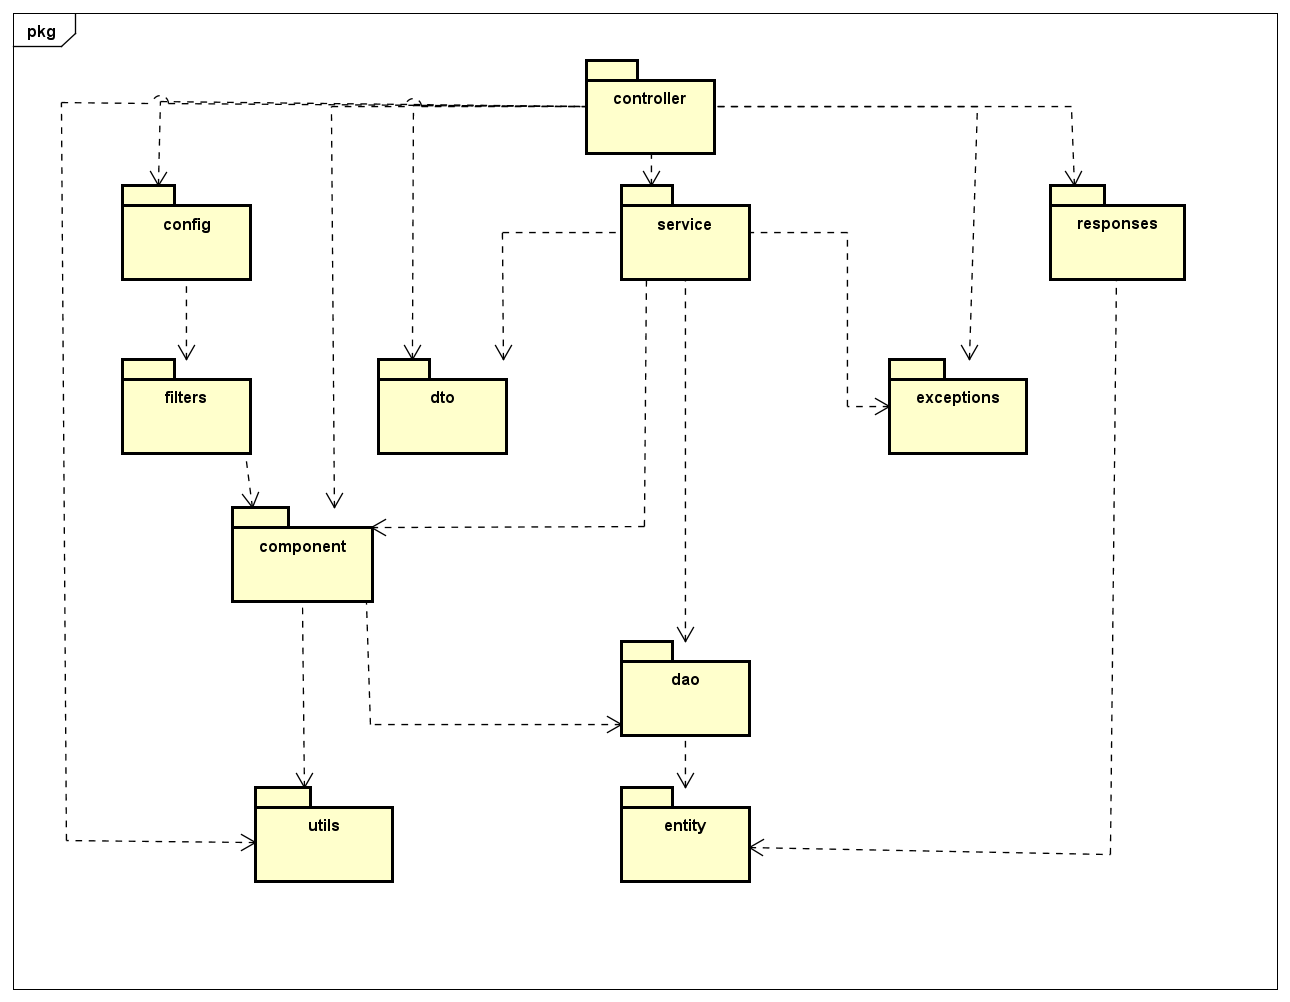
\includegraphics{Hinhve/sơ đồ gói tổng quát.png}
    }
    \caption{Ví dụ biểu đồ phụ thuộc gói}
    \label{fig:Fig1}
\end{figure}

Trong biểu đồ Hình \ref{fig:Fig1a}  đưa ra thiết kế tổng quát cho bên phía FE bao gồm:

\textbf{FE component}:
\begin{enumerate}
    \item[(i)] \textbf{Mục đích}: Noi chứa các component cũng là các thành phần màn hình của hệ thống.
    \item[(ii)] \textbf{Phụ thuộc}: Phụ thuộc vào FE Service, common, model, validator, guard và interceptor. 
\end{enumerate}

\textbf{FE service}:
\begin{enumerate}
    \item[(i)] \textbf{Mục đích}: Nơi chứa các service thực hiện về mặt logic, cũng như gọi tới các api ở bên Controller của phía BE.
    \item[(ii)] \textbf{Phụ thuộc}: Phụ thuộc vào Controller bên phía BE và common.
\end{enumerate}

\textbf{common}:
\begin{enumerate}
    \item[(i)] \textbf{Mục đích}: Nơi chứa các thành phần dùng chung của hệ thống, bao gồm có model và các file dto.
    \item[(ii)] \textbf{Phụ thuộc}: Không phụ thuộc vào gói nào.
\end{enumerate}

\textbf{guard}:
\begin{enumerate}
    \item[(i)] \textbf{Mục đích}: Nơi chứa các file guard, có nhiệm vụ xác thực quyền hạn truy cập của từng loại người dùng.
    \item[(ii)] \textbf{Phụ thuộc}: Không phụ thuộc vào file nào.
\end{enumerate}

\textbf{FE response}:
\begin{enumerate}
    \item[(i)] \textbf{Mục đích}: Nơi chứa các lớp respones định nghĩa cho các chuẩn đầu ra của api bên phía BE.
    \item[(ii)] \textbf{Phụ thuộc}: Không phụ thuộc vào gói nào.
\end{enumerate}

\textbf{validator}:
\begin{enumerate}
    \item[(i)] \textbf{Mục đích}: Nơi chứa lớp xác thực dùng cho các biểu mẫu.
    \item[(ii)] \textbf{Phụ thuộc}: Không phụ thuộc vào gói nào.
\end{enumerate}

\textbf{interceptor}:
\begin{enumerate}
    \item[(i)] \textbf{Mục đích}: Nơi chứa lớp TokenInterceptor để chèn token vào header của các HTTP Request.
    \item[(ii)] \textbf{Phụ thuộc}: Không phụ thuộc vào gói nào.
\end{enumerate}
\begin{figure}[H]
    \centering
    \scalebox{0.5}{%
        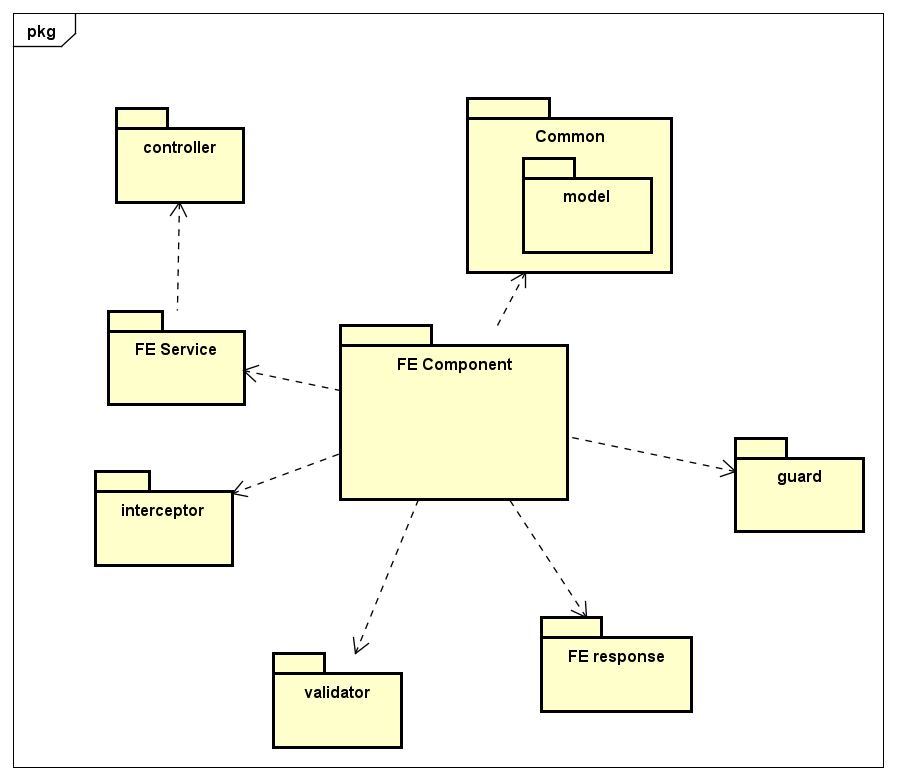
\includegraphics{Hinhve/Sơ đồ tổng quát FE.png}
    }
    \caption{Ví dụ biểu đồ phụ thuộc gói phía FE}
    \label{fig:Fig1a}
\end{figure}

\subsection{Thiết kế chi tiết gói}
% Sinh viên thiết kế và lần lượt vẽ biểu đồ thiết kế cho từng package, hoặc một nhóm các package liên quan để giải quyết một vấn đề gì đó. Khi vẽ thiết kế gói, sinh viên chỉ cần đưa tên lớp, không cần chỉ ra các thành viên phương thức và thuộc tính. SV tham khảo ví dụ minh họa trong Hình \ref{fig:Fig2}.

% Sinh viên cần vẽ rõ ràng quan hệ giữa các lớp trong biểu đồ. Các quan hệ bao gồm: phụ thuộc (dependency), kết hợp (association), kết tập (aggregation), hợp thành (composition), kế thừa (inheritance), và thực thi (implementation). Các quan hệ này đều đã được minh họa trong \ref{fig:Fig2}.

% Sau khi vẽ hình minh họa, sinh viên cần giải thích ngắn gọn về thiết kế của mình. 
\subsubsection{Biểu đồ gói Controller}

\begin{figure}[H]
    \centering
   \scalebox{0.7}{%
        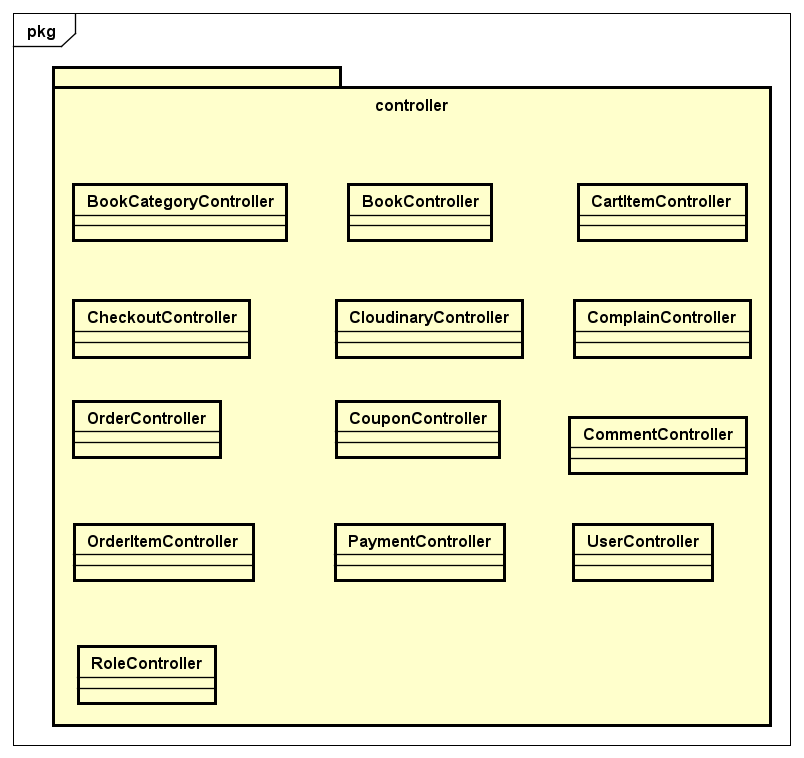
\includegraphics{Hinhve/controller Diagram.png}
    }
    \caption{Biểu đồ gói Controller}
    \label{fig:Fig2}
\end{figure}
Gói controller bao gồm các các lớp controller chịu trách nhiệm cho các tác vụ khác nhau. Các lớp Controller ở đây bao gôm:
\begin{enumerate}
    \item [(i)] \textbf{BookController}: Chịu trách nhiệm xử lý các yêu cầu về sách.
    \item [(ii)]\textbf{BookCategoryController}: Chịu trách nhiệm xử lý các yêu cầu về danh mục.
    \item[(iii)] \textbf{CartItemController}: Chịu trách nhiệm xử lý các yêu cầu về các mặt hàng trong giỏ hàng.
    \item[(iv)] \textbf{CheckoutController}: Chịu trách nhiệm xử lý yêu cầu về tạo mới đơn hàng.
    \item[(v)] \textbf{CloudinaryController}: Chịu trách nhiệm xử lý yêu cầu về đăng ảnh bìa cho sách.
    \item[(vi)] \textbf{ComplainController}: Chịu trách nhiệm xử lý các yêu cầu về hệ thống hỗ trợ.
    \item[(vii)] \textbf{CouponController}: Chịu trách nhiệm xử lý yêu cầu về tính toán khi áp dụng mã giảm giá.
    \item[(viii)] \textbf{OrderController}: Chịu trách nhiệm xử lý các yêu cầu về đơn hàng.
    \item[(ix)] \textbf{CommentController}: Chịu trách nhiệm xử lý các yêu càu về bình luận.
    \item[(x)] \textbf{OrderItemController}: Chịu trách nhiệm xử lý yêu cầu về các mặt hàng trong 1 đơn hàng.
    \item[(xi)] \textbf{PaymentController}: Chịu trách nhiệm xử lý yêu cầu về thanh toán online.
    \item[(xii)] \textbf{UserController}: Chịu trách nhiệm xử lý các yêu cầu về người dùng.
    \item[(xiii)] \textbf{RoleController}: Chịu trách nhiệm xử lý các yêu cầu về vai trò trong hệ thống.  
\end{enumerate}

\subsubsection{Biểu đồ gói Config}

\begin{figure}[H]
    \centering
   \scalebox{0.7}{%
        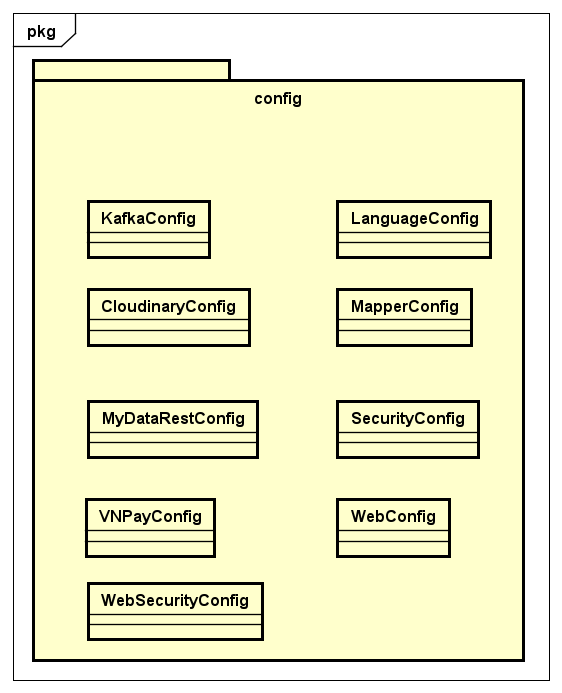
\includegraphics{Hinhve/config diagram.png}
    }
    \caption{Biểu đồ gói Config}
    \label{fig:Fig3}
\end{figure}
Gói config bao gồm các các lớp config chịu trách nhiệm cấu hình cho ứng dụng. Các lớp configr ở đây bao gôm:
\begin{enumerate}
    \item [(i)] \textbf{KafkaConfig}: Chịu trách nhiệm cấu hình veeff Kafka cho ứng dụng.
    \item [(ii)]\textbf{LanguageConfig}: Chịu trách nhiệm cấu hình phần ngôn ngữ của ứng dụng.
    \item[(iii)] \textbf{CloudinaryConfig}: Chịu trách nhiệm cấu hình  cho Cloudinary.
    \item[(iv)] \textbf{MapperConfig}: Chịu trách nhiệm cáu hình cho ModelMapper.
    \item[(v)] \textbf{MyDataRestConfig}: Chịu trách nhiệm cấu hình cho các request đọc dữ liệu của Book, BookCategory, City và Country.
    \item[(vi)] \textbf{SecurityConfig}: Chịu trách nhiệm cáu hình vè bảo mật và xác thực người dùng.
    \item[(vii)] \textbf{VNPayConfig}: Chịu trách nhiệm cáu hình cho cổng thanh toán VNPAY.
    \item[(viii)] \textbf{WebConfig}: Chịu trách nhiệm cấu hình các quy tắc CORS( Cross origin Resource Sharing).
    \item[(ix)] \textbf{WebSecurityConfig}: Chịu trách nhiệm cấu hình về bảo mật cho các đầu api của hệ thống.
\end{enumerate}

\subsubsection{Biểu đồ gói component}

\begin{figure}[H]
    \centering
   \scalebox{0.7}{%
        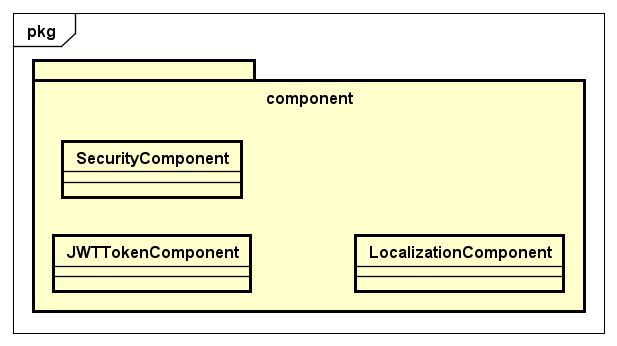
\includegraphics{Hinhve/component diagram.png}
    }
    \caption{Biểu đồ gói component}
    \label{fig:Fig4}
\end{figure}
Gói component bao gồm các lớp component chứa các thành phần dùng chung cho nhiều phần khác nhau của hệ thống. Bao gồm:
\begin{enumerate}
    \item [(i)] \textbf{SecurityComponent}: Chịu trách nhiệm lấy thông tin về người dùng hiện tại đang đăng nhập trong hệ thống.
    \item [(ii)]\textbf{JWTTokenComponent}: Chứa các hàm về Jwt Token  bao gồm khởi tạo, trích xuất Claims, kiểm tra thời hạn của Token.
    \item[(iii)] \textbf{LocalizationComponent}: Chứa hàm xử lý các tin nhắn thông báo được mã hóa sẵn.
\end{enumerate}

\subsubsection{Biểu đồ gói dao}

\begin{figure}[H]
    \centering
   \scalebox{0.6}{%
        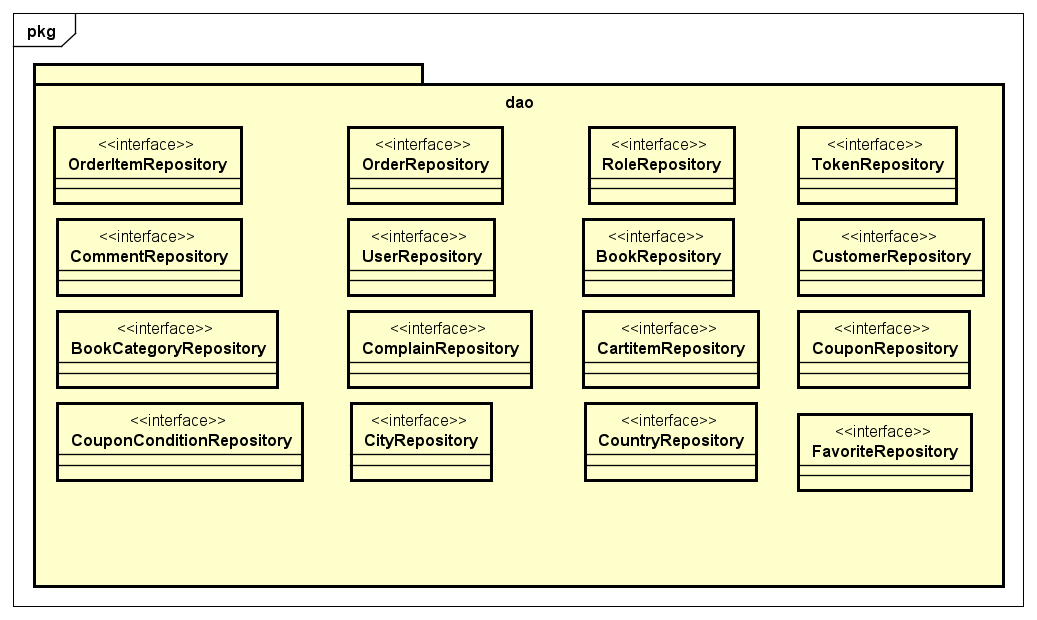
\includegraphics{Hinhve/dao diagram.png}
    }
    \caption{Biểu đồ gói dao}
    \label{fig:Fig5}
\end{figure}
Gói dao bao gồm các interface được kế thừa từ JpaRepository dùng để giao tiếp với các bảng trong cơ sở dữ liệu. Các interface ở đây bao gôm:
\begin{enumerate}
    \item [(i)] \textbf{OrderItemRepository}: Chịu trách nhiệm giao tiếp với bảng order-item..
    \item [(ii)]\textbf{OrderRepository}: Chịu trách nhiệm giao tiếp với bảng orders.
    \item[(iii)] \textbf{RoleRepository}: Chịu trách nhiệm giao tiếp với bảng role.
    \item[(iv)] \textbf{TokenRepository}: Chịu trách nhiệm giao tiếp với bảng token.
    \item[(v)] \textbf{CommentRepository}: Chịu trách nhiệm giao tiếp với bảng comment.
    \item[(vi)] \textbf{UserRepository}: Chịu trách nhiệm giao tiếp với bảng users
    \item[(vii)] \textbf{BookRepository}: Chịu trách nhiệm giao tiếp với bảng books.
    \item[(viii)] \textbf{CustomerRepository}: Chịu trách nhiệm giao tiếp với bảng customer.
    \item[(ix)] \textbf{BookCategoryRepository}: Chịu trách nhiệm giao tiếp với bảng book-category.
    \item[(x)] \textbf{ComplainRepository}: Chịu trách nhiệm giao tiếp với bảng complain.
    \item[(xi)] \textbf{CartitemRepository}: Chịu trách nhiệm giao tiếp với bảng cart-item.
    \item[(xii)] \textbf{CouponRepository}: Chịu trách nhiệm giao tiếp với bảng coupon.
    \item[(xiii)] \textbf{CouponConditionRepository.}: Chịu trách nhiệm giao tiếp với bảng coupon-condition. 
    \item[(xiv)] \textbf{CityRepository}: Chịu trách nhiệm giao tiếp với bảng city.
    \item[(xv)] \textbf{CountryRepository}: Chịu trách nhiệm giao tiếp với bảng country.
    \item[(xvi)] \textbf{FavoriteRepository}: Chịu trách nhiệm giao tiếp với bảng favorite.    
\end{enumerate}

\subsubsection{Biểu đồ gói dto}

\begin{figure}[H]
    \centering
   \scalebox{0.6}{%
        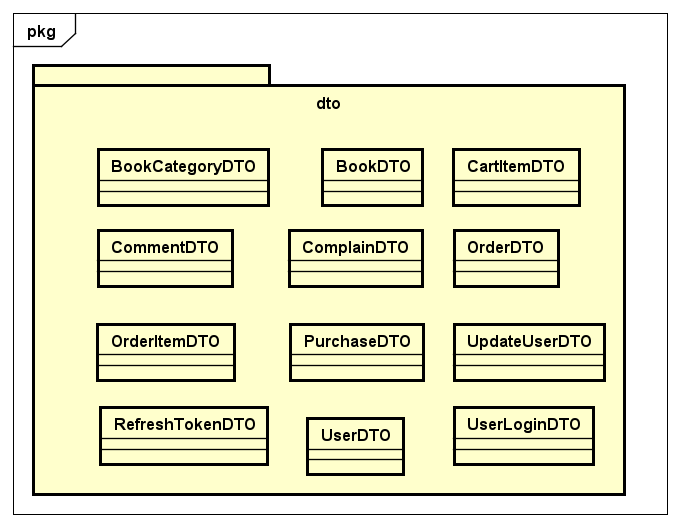
\includegraphics{Hinhve/dto diagrams.png}
    }
    \caption{Biểu đồ gói dto}
    \label{fig:Fig6}
\end{figure}
Gói dto bao gồm các lớp dto chịu trách nhiệm truyền dữ liệu, bao gồm:
\begin{enumerate}
    \item [(i)] \textbf{BookDTO}: Chịu trách nhiệm tạo đầu vào dạng Book.
    \item [(ii)]\textbf{BookCategoryDTO}: Chịu trách nhiệm tạo đầu vào dạng Book-Category.
    \item[(iii)] \textbf{CartItemDTO}: Chịu trách nhiệm tạo đầu vào dạng cart-item.
    \item[(iv)] \textbf{PurchaseDTO}: Chịu trách nhiệm tạo đầu vào dạng Purchase cho việc tạo đơn hàng.
    \item[(v)] \textbf{CommentDTO}: Chịu trách nhiệm tạo đàu vào dạng comment.
    \item[(vi)] \textbf{ComplainDTO}: Chịu trách nhiệm tạo đầu vào dạng complain.
    \item[(vii)] \textbf{OrderDTO}: Chịu trách nhiệm tạo đầu vào dạng Order.
    \item[(viii)] \textbf{OrderItemDTO}: Chịu trách nhiệm tạo đầu vào dạng Order-item.
    \item[(ix)] \textbf{UpdateUserDTO}: Chịu trách nhiệm tạo đầu vào cho việc cập nhật thông tin người dùng.
    \item[(x)] \textbf{RefreshTokenDTO}: Chịu trách nhiệm tạo đầu vào cho yêu cầu refreshToken.
    \item[(xi)] \textbf{UserDTO}: Chịu trách nhiệm tạo đầu vào cho các yêu cầu liên quan tới người dùng.
    \item[(xii)] \textbf{UserLoginDTO}: Chịu trách nhiệm tạo đầu vào cho yêu cầu đăng nhập.
\end{enumerate}

\subsubsection{Biểu đồ gói entity}

\begin{figure}[H]
    \centering
   \scalebox{0.6}{%
        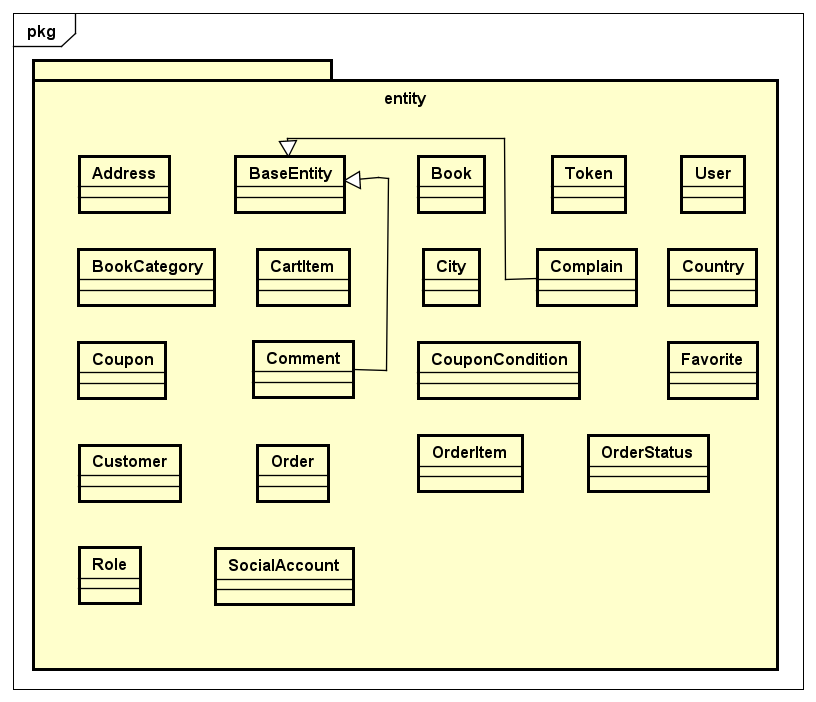
\includegraphics{Hinhve/entity diagram.png}
    }
    \caption{Biểu đồ gói entity}
    \label{fig:Fig7}
\end{figure}
Gói entity bao gồm các entity đại diện cho các bảng trong cơ sở dữ liệu. Gói entity bao gồm:
\begin{enumerate}
    \item [(i)] \textbf{Address}: Đại diện cho bảng Address.
    \item [(ii)]\textbf{BaseEntity}: Không đại diện cho bảng nào, là lớp cơ sở dể cho một số lớp khác kế thừa.
    \item[(iii)] \textbf{Book}: Đại diện cho bảng books.
    \item[(iv)] \textbf{Token}:Đại diện cho bảng token.
    \item[(v)] \textbf{User}: Đại diện cho bảng users.
    \item[(vi)] \textbf{BookCategory}: Đại diện cho bảng book-categories.
    \item[(vii)] \textbf{CartItem}:Đại diện cho bảng cart-item.
    \item[(viii)] \textbf{City}: Đại diện cho bảng city.
    \item[(ix)] \textbf{Complain}: Đại diện cho bảng complains, kế thừa BaseEntity..
    \item[(x)] \textbf{Country}: Đại diện cho bảng country.
    \item[(xi)] \textbf{Coupon}:Đại diện cho bảng coupon.
    \item[(xii)] \textbf{Comment}: Đại diện cho bảng comments, kế thừa BaseEntity.
    \item [(xiii)] \textbf{CouponCondition}: Đại diện cho bảng coupon-condition.
    \item[(xiv)] \textbf{Favorite}: Đại diện cho bảng favorite.
    \item[(xv)] \textbf{Customer}: Đại diện cho bảng customer.
    \item[(xvi)] \textbf{Order}: Đại diện cho bảng orders.
    \item[(xvii)] \textbf{OrderItem}: Đại diện cho bảng order-items.
    \item[(xviii)] \textbf{OrderStatus}: Không đại diện cho bảng nào, chứa các giá trị của trạng thái đơn hàng.
    \item[(xix)] \textbf{Role}: Đại diện cho bảng role.
    \item[(xx)] \textbf{SocialAccount}: Đại diện cho bảng social-account.
\end{enumerate}

\subsubsection{Biểu đồ gói exceptions}

\begin{figure}[H]
    \centering
   \scalebox{0.6}{%
        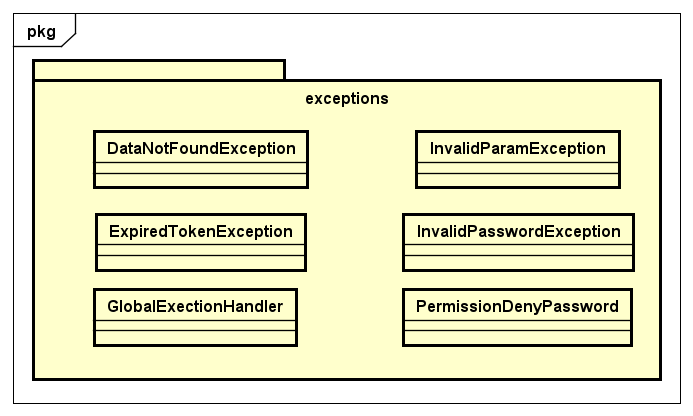
\includegraphics{Hinhve/exception diagram.png}
    }
    \caption{Biểu đồ gói exceptions}
    \label{fig:Fig7}
\end{figure}
Gói exceptions bao gồm các lớp exceptions chứa các lỗi ngoại lê, bao gồm:
\begin{enumerate}
    \item [(i)] \textbf{DataNotFound}:Kế thừa từ Exception, chứa thông tin lỗi DataNotFoundException.
    \item [(ii)]\textbf{InvalidParamException}::Kế thừa từ Exception, chứa thông tin lỗi InvalidParamException.
    \item[(iii)] \textbf{ExpiredTokenException}: Kế thừa từ Exception, chứa thông tin lỗi ExpiredTokenExeption.
    \item[(iv)] \textbf{InvalidPasswordException}:Kế thừa từ Exception, chứa thông tin lỗi InvalidPasswordException.
    \item[(v)] \textbf{PermissionDenyException}: Kế thừa từ Exception, chứa thông tin lỗi PermissionDenyException.
    \item[(vi)] \textbf{GlobalExceptionHandler}: Xử lý các ngoại lệ.
\end{enumerate}

\subsubsection{Biểu đồ gói filter}
\begin{figure}[H]
    \centering
   \scalebox{1}{%
        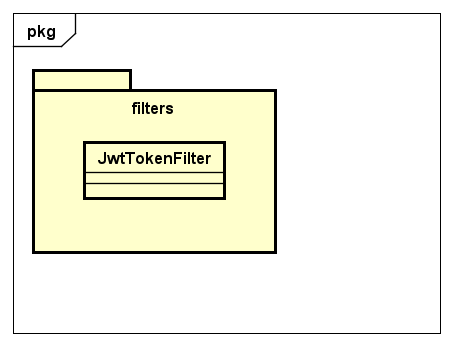
\includegraphics{Hinhve/filters diagram.png}
    }
    \caption{Biểu đồ gói filters}
    \label{fig:Fig8}
\end{figure}
Gói filters chứa bộ lọc để xử lý các yêu cầu HTTP trước khi đến Controller. Gói filters chi chứa 1 class:
\textbf{JwtTokenFilter}: Chỉ định xem các đầu api nào cần có jwt token để xác thực.

\subsubsection{Biểu đồ gói respones}

\begin{figure}[H]
    \centering
   \scalebox{0.5}{%
        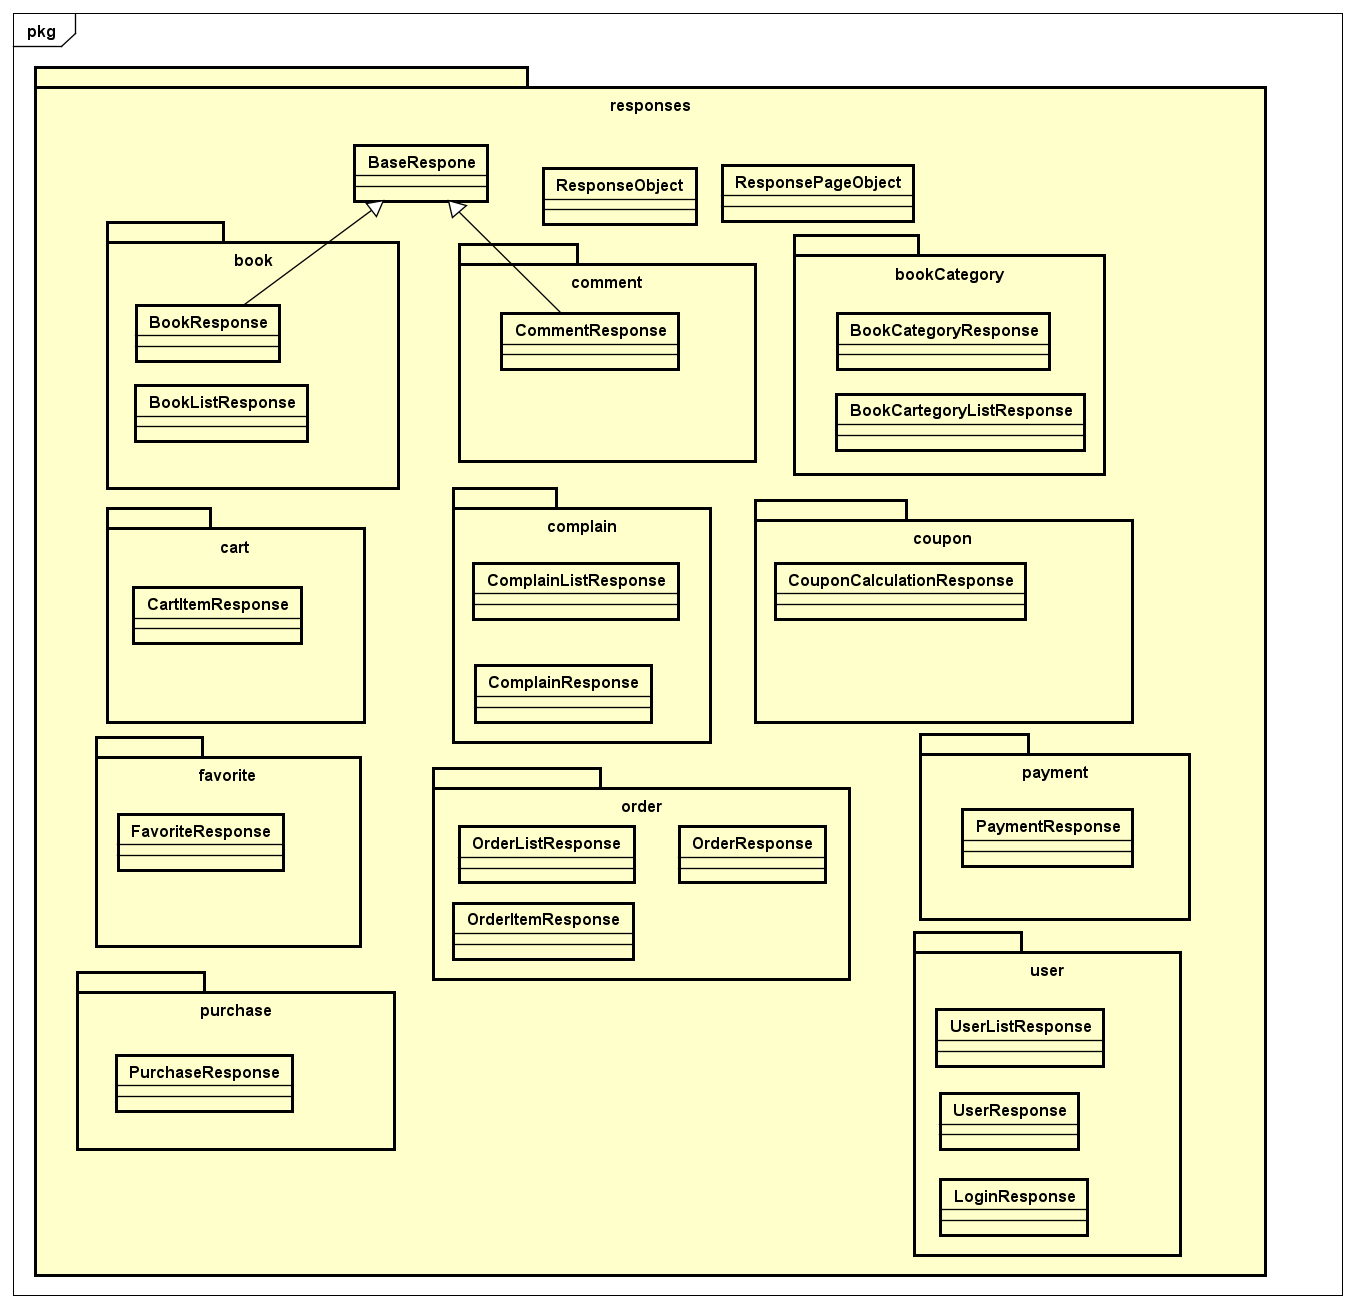
\includegraphics{Hinhve/responses diagram.png}
    }
    \caption{Biểu đồ gói responses}
    \label{fig:Fig7}
\end{figure}
Gói responses  bao gồm các lớp responese định nghĩa kiểu trả về chuẩn của hệ thống:
\begin{enumerate}
    \item [(i)] \textbf{BaseResponse}: Lớp response cơ bản, dùng cho một số lớp khác kế thừa.
    \item [(ii)]\textbf{ResponseObject}: Lớp Response chung, các api thường trả về ResponseObject với data là các lớp Response khác.
    \item[(iii)] \textbf{ResponsePageObject}:Giống với ResponseObject nhưng có thêm thông tin TotalPage.
    \item[(iv)] \textbf{user}: Gồm 3 lớp là LoginResponse, UserResponse và UserListResponse.
    \item[(v)] \textbf{book}: Bao gồm có 2 lớp là BookResponse kế thừa từ BaseResponse, và BookListResponse.
    \item[(vi)] \textbf{comment}: Gồm 1 lớp commentResponse kế thừa từ BaseResponse.
    \item[(vii)] \textbf{bookCategory}:Gồm lớp BookCategoryResponse và BookCategoryListReponse.
     \item[(viii)] \textbf{purchase}: Gồm 1 lớp PurchaseResponse.
    \item[(ix)] \textbf{cart}: Gồm 1 lớp CartItemResponse.
    \item[(x)] \textbf{complain}: Gồm 2 lớp ComplainResponse và ComplainListResponse.
    \item[(xi)] \textbf{coupon}:Gồm 1 lớp CouponCalculationResponse.
    \item[(xii)] \textbf{favorite}: Gồm 1 lớp FavoriteResponse.
    \item [(xiii)] \textbf{order}: Gồm 3 lớp OrderItemResponse, OrderResponse và OrderListResponse.
    \item[(xiv)] \textbf{payment}: Gồm 1 lớp PaymentResponse.
    
\end{enumerate}

\subsubsection{Biểu đồ gói service}

\begin{figure}[H]
    \centering
   \scalebox{0.5}{%
        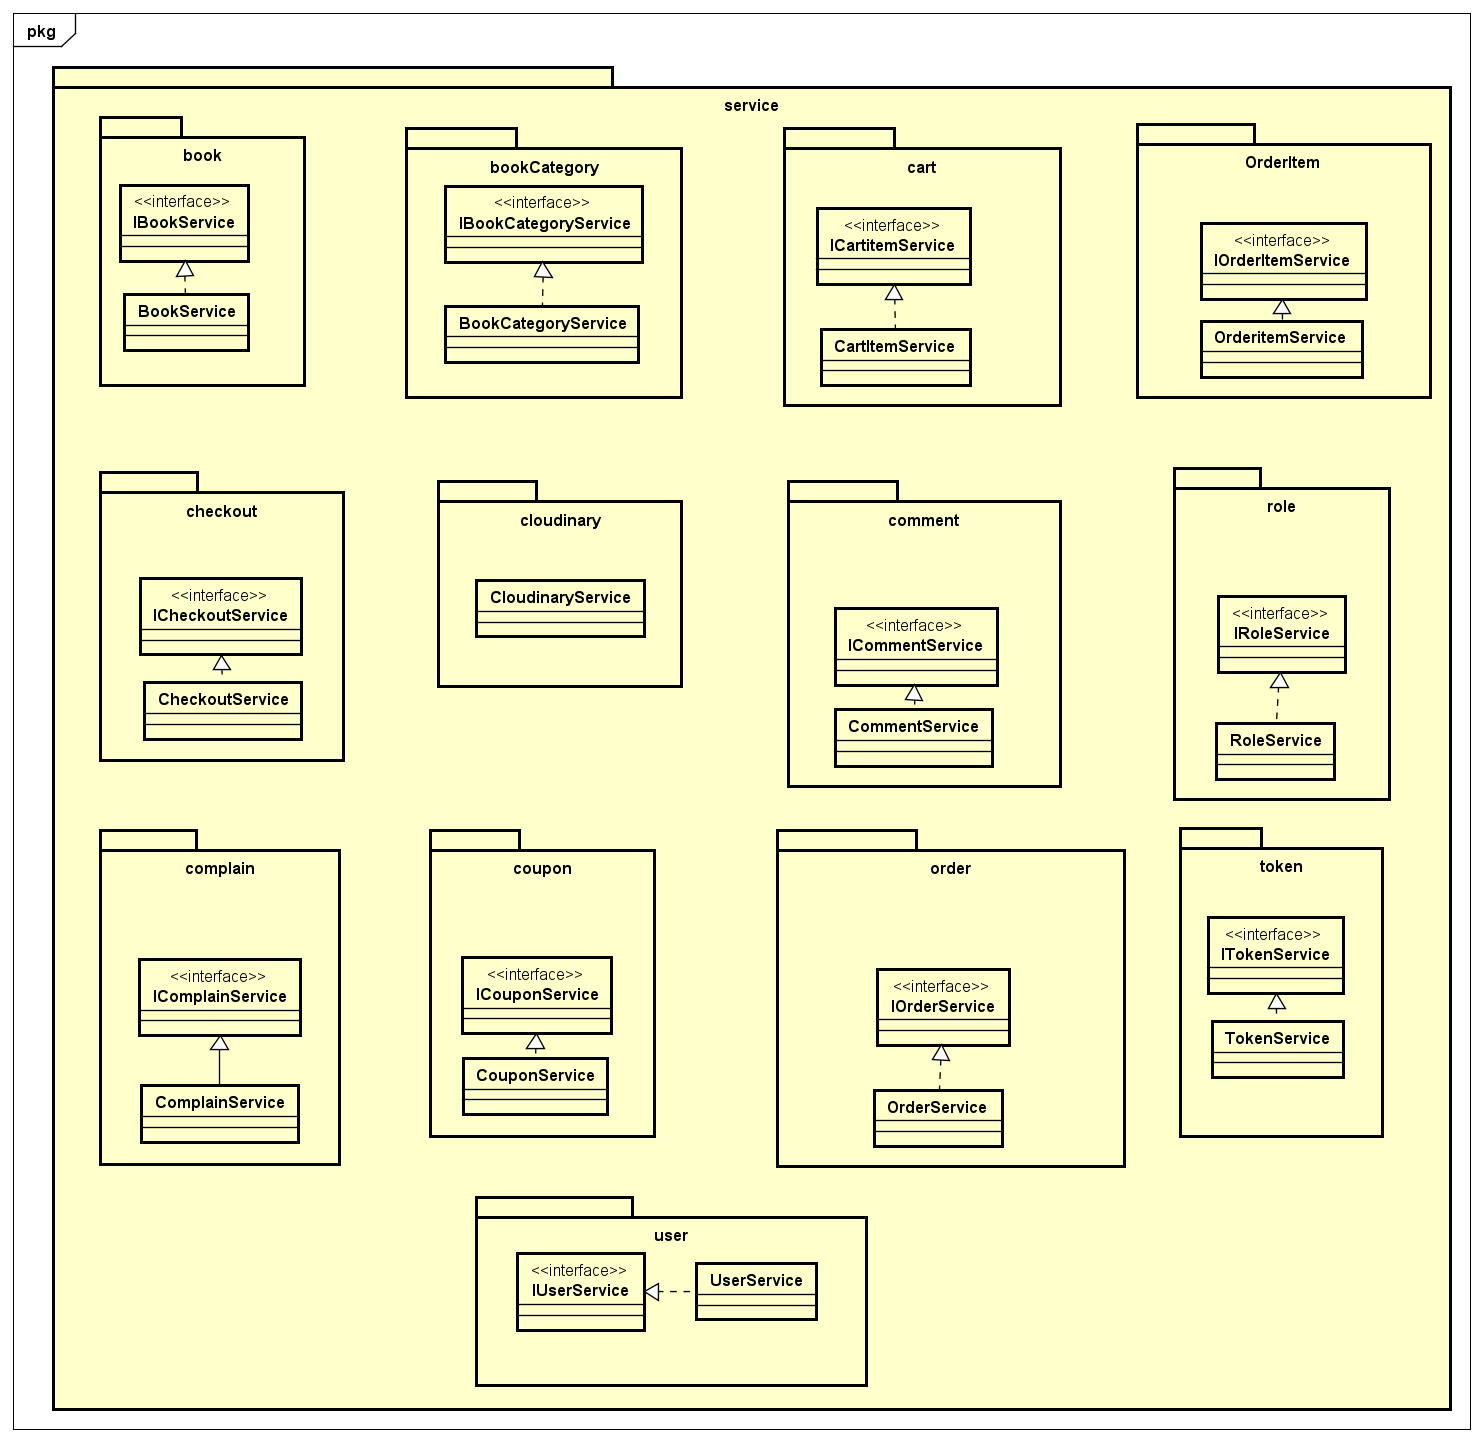
\includegraphics{Hinhve/service diagram.png}
    }
    \caption{Biểu đồ gói service}
    \label{fig:Fig7}
\end{figure}
Gói service bao gồm các gói chứa các lớp và interface tương ứng nhau trong quá trình xử lý logic nghiệp vụ. Các gói trong service bao gồm:
\begin{enumerate}
    \item [(i)] \textbf{book}: Bao gồm interface IBookService và lớp BookService thực thi IBookService.
    \item [(ii)]\textbf{bookCategory}: bao gồm interface IBookCategoryService và lớp thực thi.
    \item[(iii)] \textbf{cart}:Bao gồm interface ICartItemService và lớp thực thi.
    \item[(iv)] \textbf{orderItem}: Bao gồm interface IOrderItemService và lớp thực thi.
    \item[(v)] \textbf{checkout}: Bao gồm interface ICheckoutService và lớp thực thi.
    \item[(vi)] \textbf{comment}: Bao gồm interface ICommentService và lớp thực thi.
    \item[(vii)] \textbf{cloudinary}:Gồm 1 lớp CloudinaryService.
     \item[(viii)] \textbf{role}: Bao gồm interface IRoleService và lớp thực thi.
    \item[(ix)] \textbf{token}: Bao gồm interface ITokenService và lớp thực thi.
    \item[(x)] \textbf{complain}: Gồm interface IComplainService và lớp thực thi
    \item[(xi)] \textbf{coupon}:Gồm interface ICouponService và lớp thực thi.
    \item[(xii)] \textbf{user}: Gồm interface IUserService và lớp thực thi.
    \item [(xiii)] \textbf{order}: Gồm interface IOrderService và lớp thực thi.   
\end{enumerate}

\subsubsection{Biểu đồ gói utils}

\begin{figure}[H]
    \centering
   \scalebox{1}{%
        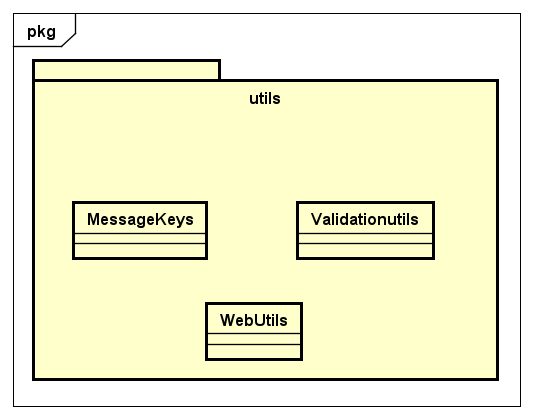
\includegraphics{Hinhve/utils diagram.png}
    }
    \caption{Biểu đồ gói utils}
    \label{fig:Fig8}
\end{figure}
Gói utils các lớp utils là các thành phần tiện tích của hệ thống. Bao gồm:
\begin{enumerate}
    \item [(i)] \textbf{MessageKeys}: Chứa các keys và Message tương ứng.
    \item [(ii)]\textbf{ValidationUtils}: Chứa các hàm xác thực số điện thoại và email.
    \item[(iii)] \textbf{WebUtils}: Chứa hàm sử dụng để lấy đối tượng HttpServletRequest.
\end{enumerate}
\section{Thiết kế chi tiết}
\subsection{Thiết kế giao diện}
% Phần này có độ dài từ hai đến ba trang. Sinh viên đặc tả thông tin về màn hình mà ứng dụng của mình hướng tới, bao gồm độ phân giải màn hình, kích thước màn hình, số lượng màu sắc hỗ trợ, v.v. Tiếp đến, sinh viên đưa ra các thống nhất/chuẩn hóa của mình khi thiết kế giao diện như thiết kế nút, điều khiển, vị trí hiển thị thông điệp phản hồi, phối màu, v.v. Sau cùng sinh viên đưa ra một số hình ảnh minh họa thiết kế giao diện cho các chức năng quan trọng nhất. Lưu ý, sinh viên không nhầm lẫn giao diện thiết kế với giao diện của sản phẩm sau cùng.
\subsubsection{thông số của giao diện}
Các thông số màn hình và thiết kế giao diện mà hệ thống hướng tới: 
\begin{enumerate}
    \item[(i)] Giao diện đơn giản, thân thiện với người dùng.
    \item[(ii)] Độ phân giải màn hình là 1920 x 1080.
    \item[(iii)] Tỉ lệ màn hình là 16/9.
    \item[(iv)] Các thành phần giao diện được bố trí hợp lí, cân đối.
    \item[(v)] Các thành phần giao diện thể hiện rõ chức năng mà hệ thống hướng tới. 
\end{enumerate}


\subsubsection{Một số hình ảnh minh họa}

\begin{figure}[H]
    \centering
    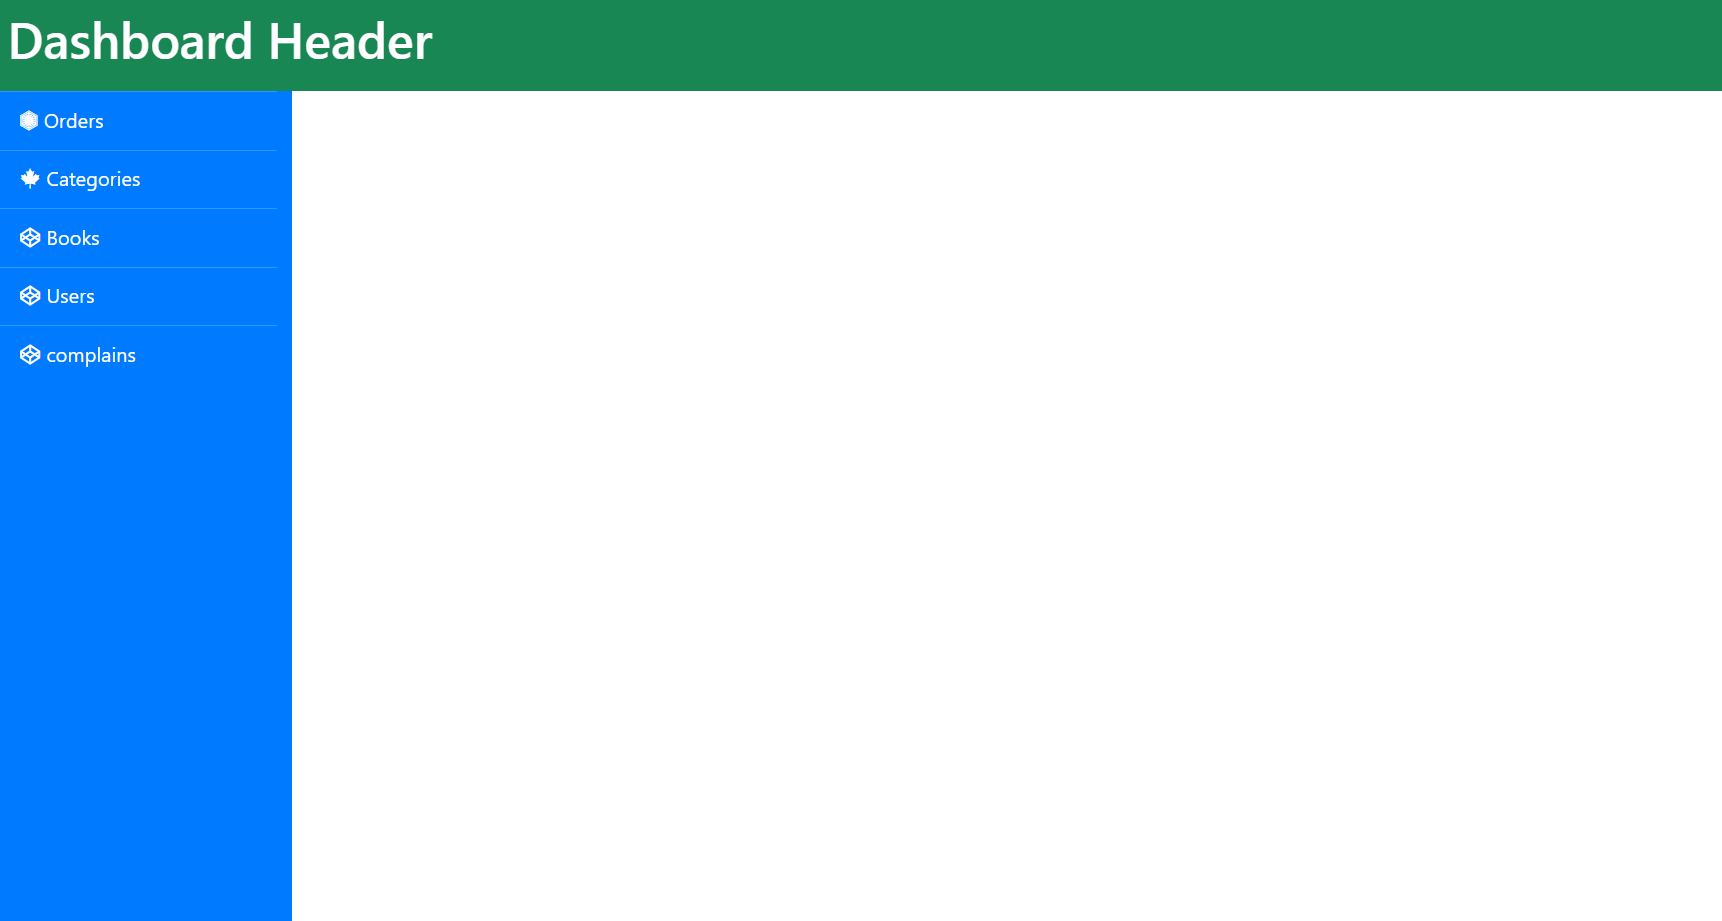
\includegraphics[width=1\linewidth]{Hinhve/admin.png}
    \caption{hình ảnh minh họa trang Admin}
    \label{fig:admin}
\end{figure}

\begin{figure}[H]
    \centering
    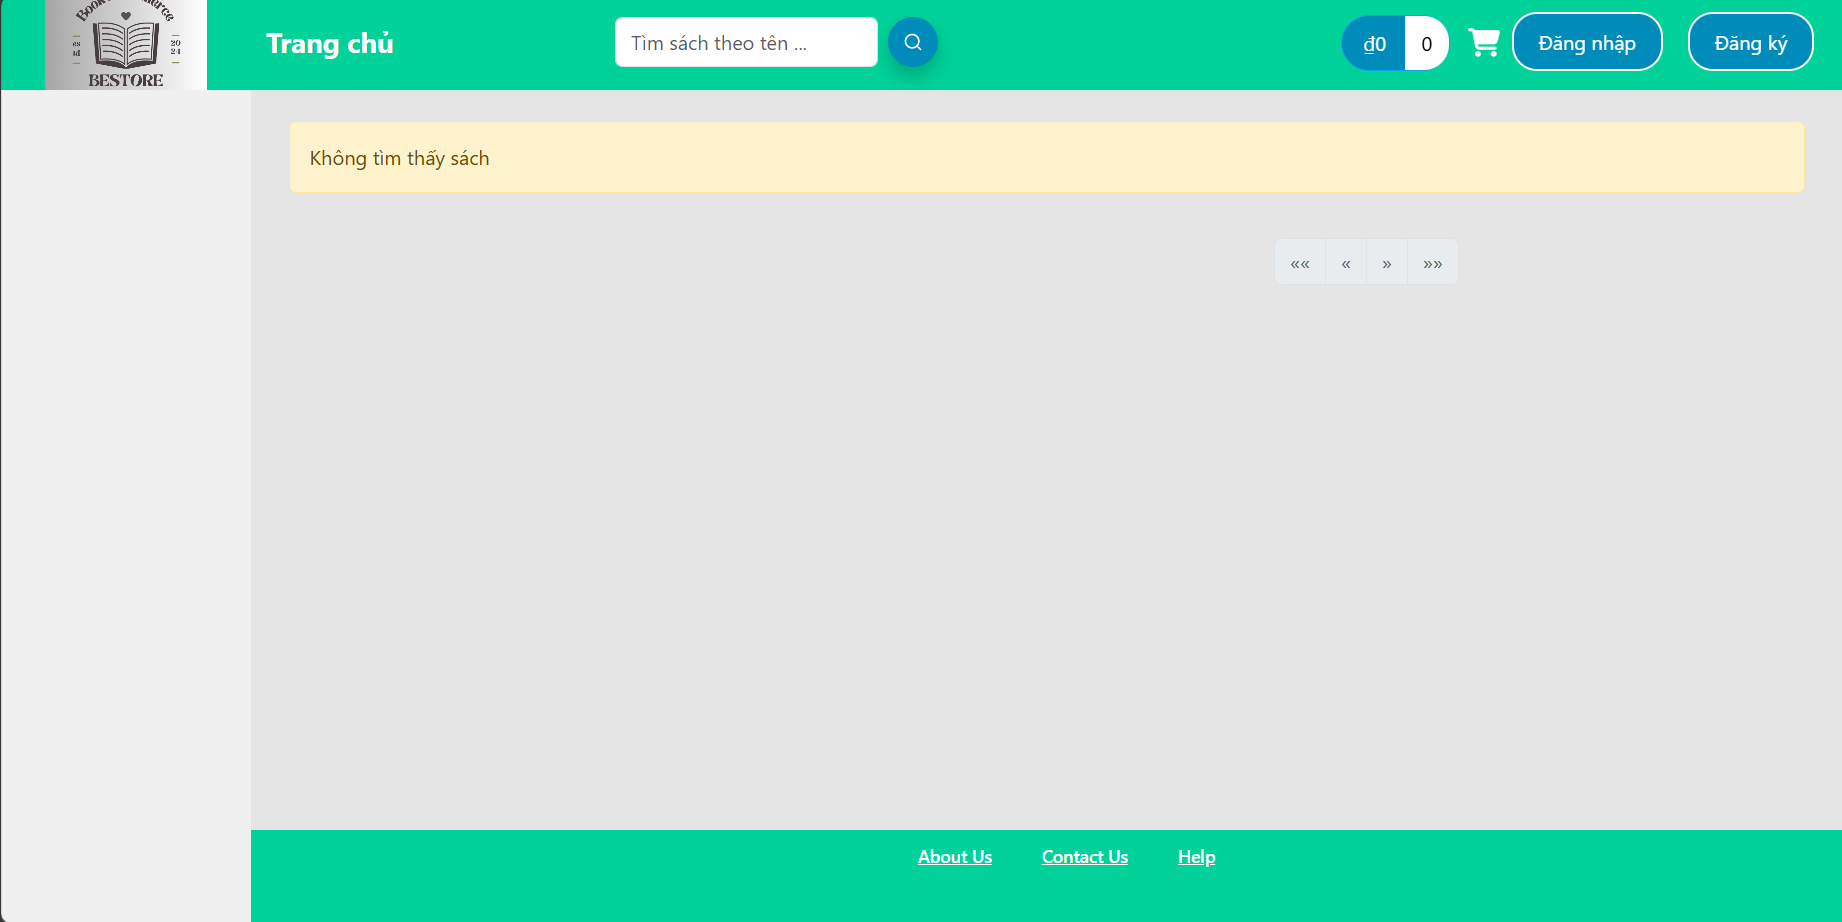
\includegraphics[width=1\linewidth]{Hinhve/home.png}
    \caption{Hình ảnh minh họa trang chủ}
    \label{fig:home}
\end{figure}

\subsection{Thiết kế lớp}

\subsubsection{Lớp Entity Book}

\begin{enumerate}
    \item[(i)] \textbf{Thuộc tính}:\\
    \begin{NiceTabular}{|c|c|c|}[hvlines]
\textbf{STT} & \textbf{Tên thuộc tính} & \textbf{Kiểu dữ liệu} \\
\hline
1  & id             & Long      \\
2  & title          & String    \\
3  & authors        & String    \\
4  & description    & String    \\
5  & publisher      & String    \\
6  & category       & BookCategory \\
7  & language       & String    \\
8  & thumbnail      & String    \\
9  & unitPrice      & double    \\
10 & active         & boolean   \\
11 & unitsInStock   & int       \\
12 & publishedDate  & Date      \\
13 & dateCreated    & Date      \\
14 & lastUpdated    & Date      \\
\end{NiceTabular}

    \item[(ii)] \textbf{Phương thức}:\\
    \begin{NiceTabular}{|c|c|c|}[hvlines]

\textbf{STT} & \textbf{Tên phương thức} & \textbf{Kiểu dữ liệu trả về} \\
\hline
1  & getId()                  & Long      \\
2  & setId(id: Long)          & void      \\
3  & getTitle()               & String    \\
4  & setTitle(title: String)  & void      \\
5  & getAuthors()             & String    \\
6  & setAuthors(authors: String) & void \\
7  & getDescription()         & String    \\
8  & setDescription(description: String) & void \\
9  & getPublisher()           & String    \\
10 & setPublisher(publisher: String) & void \\
11 & getCategory()            & BookCategory \\
12 & setCategory(category: BookCategory) & void \\
13 & getLanguage()            & String    \\
14 & setLanguage(language: String) & void \\
15 & getThumbnail()           & String    \\
16 & setThumbnail(thumbnail: String) & void \\
17 & getUnitPrice()           & double    \\
18 & setUnitPrice(unitPrice: double) & void \\
19 & isActive()               & boolean   \\
20 & setActive(active: boolean) & void \\
21 & getUnitsInStock()        & int       \\
22 & setUnitsInStock(unitsInStock: int) & void \\
23 & getPublishedDate()       & Date      \\
24 & setPublishedDate(publishedDate: Date) & void \\
25 & getDateCreated()         & Date      \\
26 & getLastUpdated()         & Date      \\
\end{NiceTabular}   
\end{enumerate}

\subsubsection{Lớp Entity User}

\begin{enumerate}
    \item[(i)] \textbf{Thuộc tính}:\\
    \begin{NiceTabular}{|c|c|c|}[hvlines]
\textbf{STT} & \textbf{Tên thuộc tính} & \textbf{Kiểu dữ liệu} \\
\hline
1  & id                  & Long    \\
2  & account             & String  \\
3  & password            & String  \\
4  & username            & String  \\
5  & phoneNumber         & String  \\
6  & email               & String  \\
7  & dateOfBirth         & Date    \\
8  & facebookAccountId   & int     \\
9  & googleAccountId     & int     \\
10 & active              & boolean \\
11 & role                & Role    \\
\end{NiceTabular}

    \item[(ii)] \textbf{Phương thức}:\\
    \begin{NiceTabular}{|c|c|c|}[hvlines]
\textbf{STT} & \textbf{Tên phương thức} & \textbf{Kiểu dữ liệu trả về} \\
\hline
1  & getId()                    & Long    \\
2  & setId(id: Long)            & void    \\
3  & getAccount()               & String  \\
4  & setAccount(account: String) & void \\
5  & getPassword()              & String  \\
6  & setPassword(password: String) & void \\
7  & getUsername()              & String  \\
8  & setUsername(username: String) & void \\
9  & getPhoneNumber()           & String  \\
10 & setPhoneNumber(phoneNumber: String) & void \\
11 & getEmail()                 & String  \\
12 & setEmail(email: String)    & void    \\
13 & getDateOfBirth()           & Date    \\
14 & setDateOfBirth(dateOfBirth: Date) & void \\
15 & getFacebookAccountId()     & int     \\
16 & setFacebookAccountId(facebookAccountId: int) & void \\
17 & getGoogleAccountId()       & int     \\
18 & setGoogleAccountId(googleAccountId: int) & void \\
19 & isActive()                 & boolean \\
20 & setActive(active: boolean) & void    \\
21 & getRole()                  & Role    \\
22 & setRole(role: Role)        & void    \\
23 & getAuthorities()           & Collection<? extends GrantedAuthority> \\
24 & isAccountNonExpired()      & boolean \\
25 & isAccountNonLocked()       & boolean \\
26 & isCredentialsNonExpired()  & boolean \\
27 & isEnabled()                & boolean \\
28 & getUsername()              & String  \\
\end{NiceTabular}
\end{enumerate}


\subsubsection{Lớp Entity Order}
\begin{enumerate}
    \item[(i)] \textbf{Thuộc tính}:\\
    \begin{NiceTabular}{|c|c|c|}[hvlines]
\textbf{STT} & \textbf{Tên thuộc tính} & \textbf{Kiểu dữ liệu} \\
\hline
1  & id                    & Long        \\
2  & orderTrackingNumber   & String      \\
3  & totalQuantity         & Integer     \\
4  & totalPrice            & Double      \\
5  & status                & String      \\
6  & dateCreated           & Date        \\
7  & lastUpdated           & Date        \\
8  & orderItems            & Set<OrderItem> \\
9  & customer              & Customer    \\
10 & shippingAddress       & Address     \\
11 & userId                & Long        \\
12 & paymentMethod         & String      \\
13 & shippingDate          & Date        \\
14 & shippingMethod        & String      \\
15 & active                & Boolean     \\
16 & coupon                & Coupon      \\
\end{NiceTabular}

    \item[(ii)] \textbf{Phương thức}:\\
    \begin{NiceTabular}{|c|c|c|}[hvlines]
\textbf{STT} & \textbf{Tên phương thức} & \textbf{Kiểu dữ liệu trả về} \\
\hline
1  & getId()                             & Long        \\
2  & setId(id: Long)                     & void        \\
3  & getOrderTrackingNumber()            & String      \\
4  & setOrderTrackingNumber(orderTrackingNumber: String) & void \\
5  & getTotalQuantity()                  & Integer     \\
6  & setTotalQuantity(totalQuantity: Integer) & void \\
7  & getTotalPrice()                     & Double      \\
8  & setTotalPrice(totalPrice: Double)   & void        \\
9  & getStatus()                         & String      \\
10 & setStatus(status: String)           & void        \\
11 & getDateCreated()                    & Date        \\
12 & getLastUpdated()                    & Date        \\
13 & getOrderItems()                     & Set<OrderItem> \\
14 & setOrderItems(orderItems: Set<OrderItem>) & void \\
15 & getCustomer()                       & Customer    \\
16 & setCustomer(customer: Customer)     & void        \\
17 & getShippingAddress()                & Address     \\
18 & setShippingAddress(shippingAddress: Address) & void \\
19 & getUserId()                         & Long        \\
20 & setUserId(userId: Long)             & void        \\
21 & getPaymentMethod()                  & String      \\
22 & setPaymentMethod(paymentMethod: String) & void \\
23 & getShippingDate()                   & Date        \\
24 & setShippingDate(shippingDate: Date) & void        \\
25 & getShippingMethod()                 & String      \\
26 & setShippingMethod(shippingMethod: String) & void \\
27 & isActive()                          & Boolean     \\
28 & setActive(active: Boolean)          & void        \\
29 & getCoupon()                         & Coupon      \\
30 & setCoupon(coupon: Coupon)           & void        \\
31 & add(item: OrderItem)                & void        \\
\end{NiceTabular}
\end{enumerate}



\subsubsection{Biểu đồ trình tự cho usecase "Đặt hàng trực tuyến" và "thanh toán online"}
\begin{figure}[H]
    \centering
        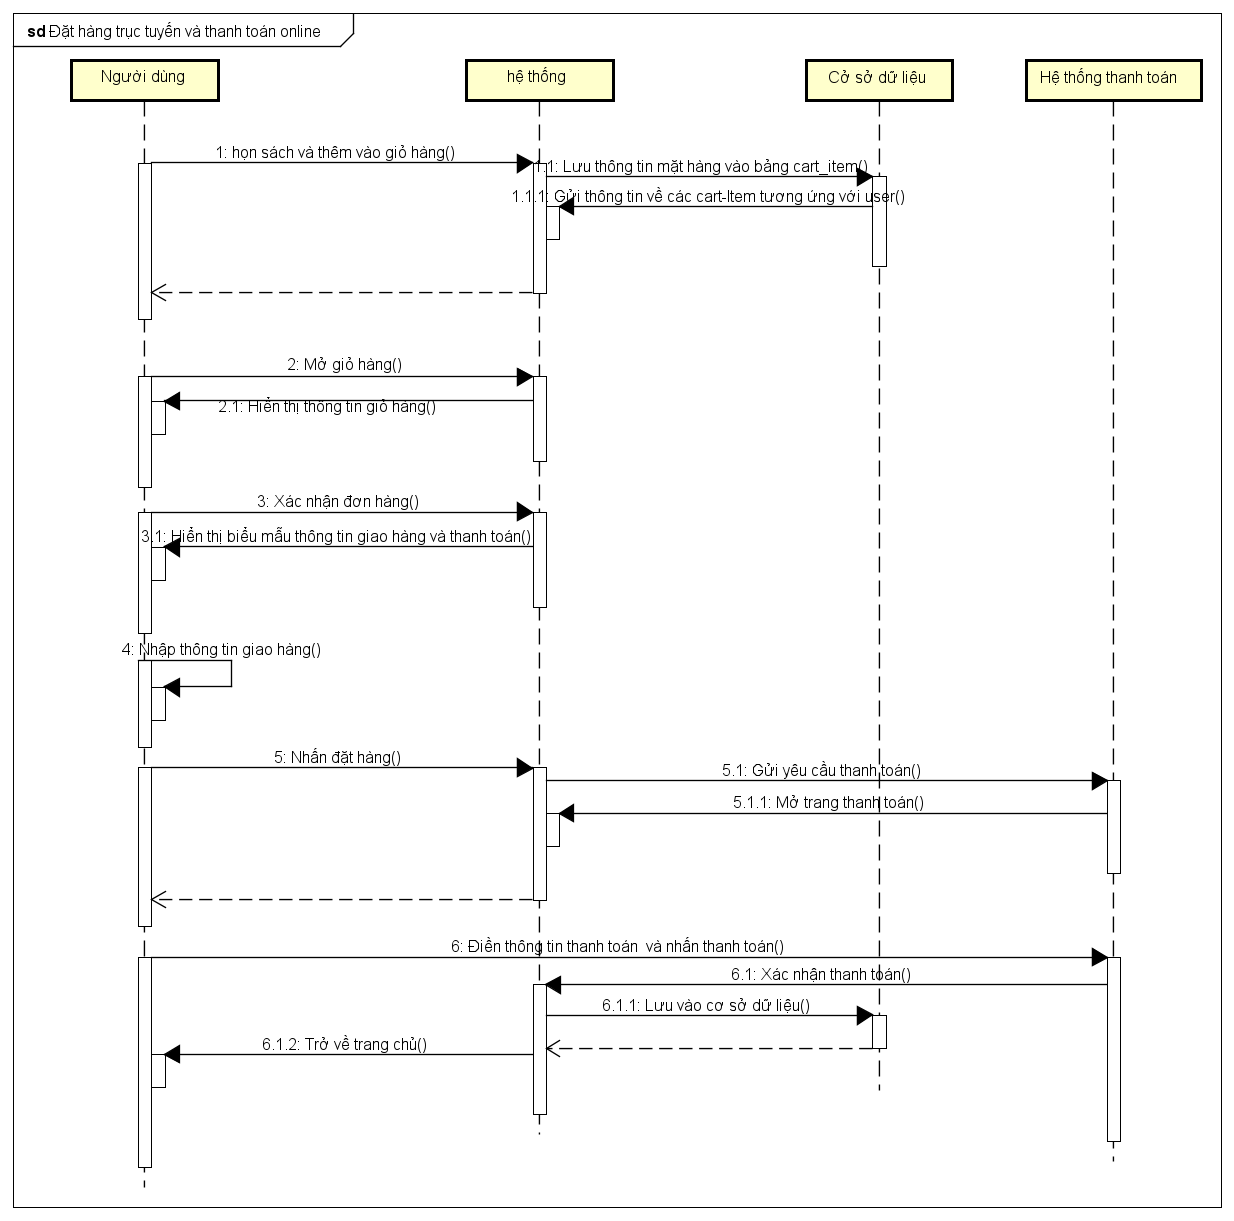
\includegraphics[width=1\textwidth]{Hinhve/Đặt hàng trục tuyến và thanh toán online.png}
    \caption{Biểu đồ trình tự cho usecase "Đặt hàng trực tuyến" và "thanh toán online"}
    \label{fig:Fig10}
\end{figure}

\subsubsection{Biểu đồ trình tự cho usecase "Thêm sách"}
\begin{figure}[H]
    \centering
        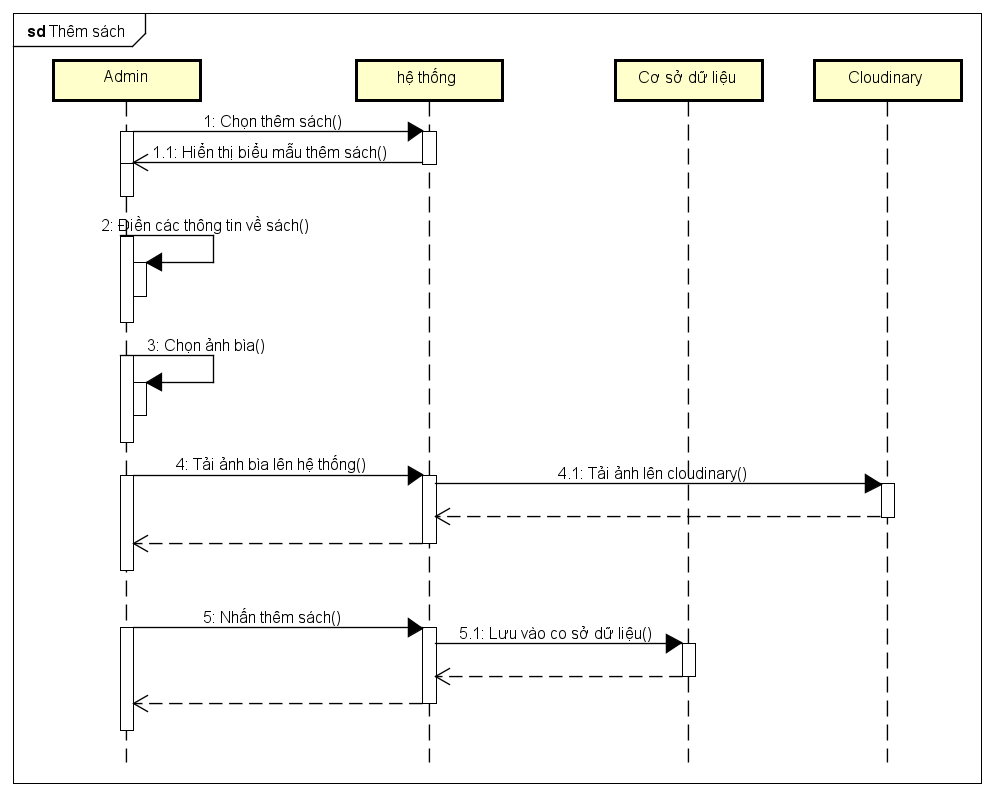
\includegraphics[width=1\textwidth]{Hinhve/Thêm sách.png}
    \caption{Biểu đồ trình tự cho usecase "Thêm sách"}
    \label{fig:Fig11}
\end{figure}

\subsection{Thiết kế cơ sở dữ liệu}

\begin{figure}[H]
    \centering
        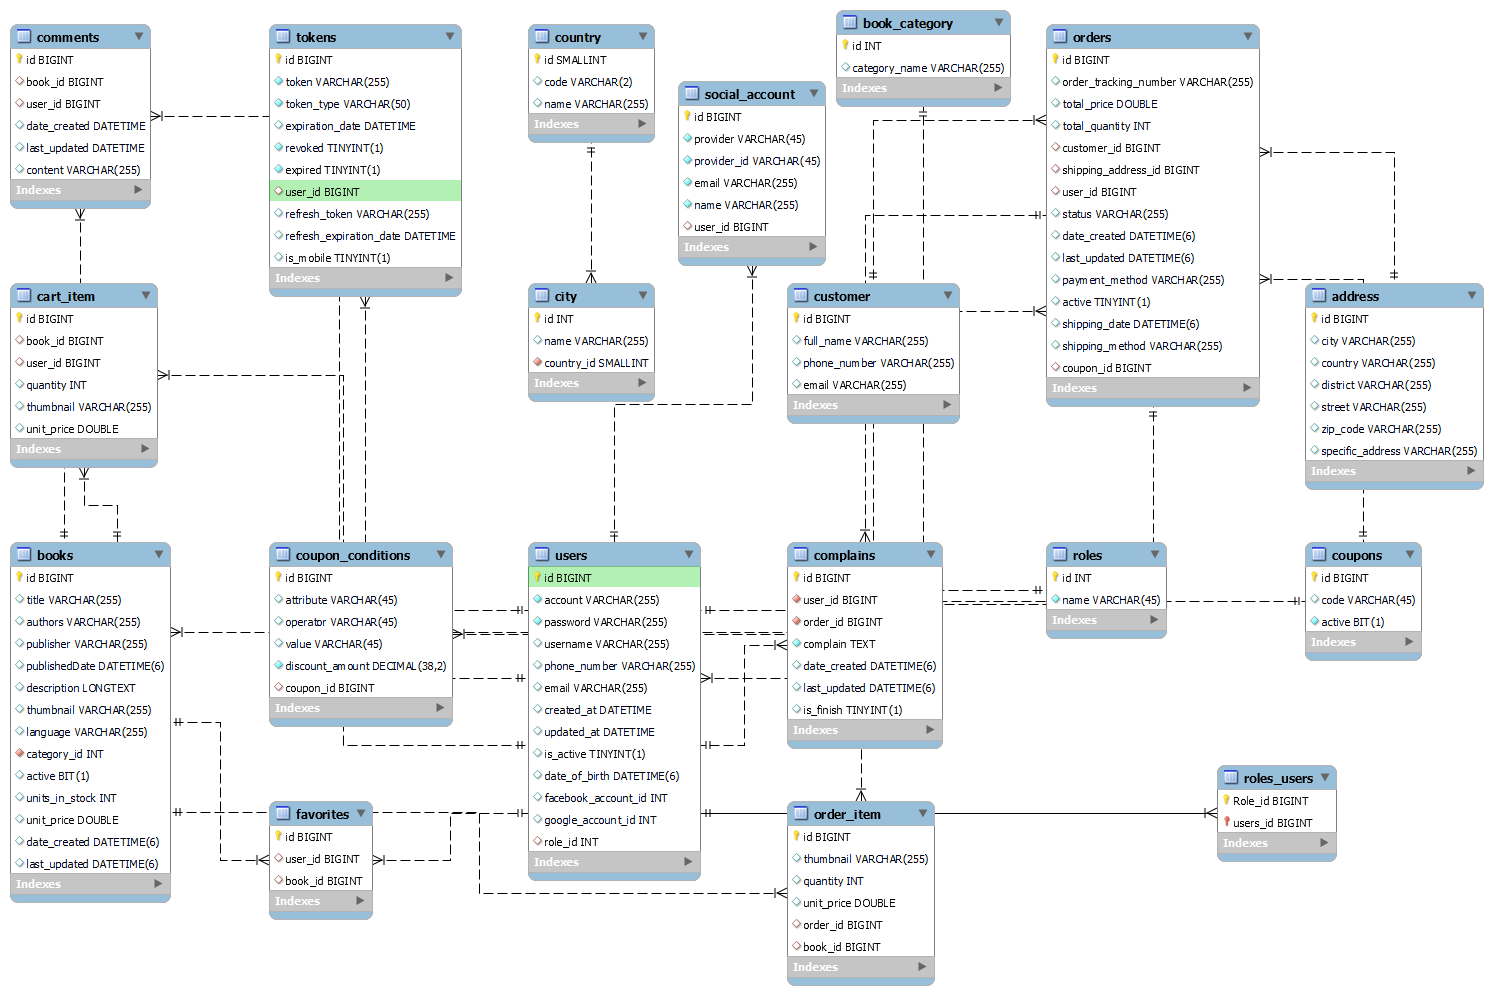
\includegraphics[width=1\textwidth]{Hinhve/database.png}
    \caption{Biểu đồ thực thể liên kết}
    \label{fig:Fig9}
\end{figure}

\subsubsection{Các Thực Thể (Entities) và Thuộc Tính (Attributes)}
\begin{enumerate}
    \item[(i)] \textbf{comments}
    % \begin{enumerate}
    %     \item[(i)] \textit{id}
    %     \item[(ii)] \textit{book\_id}
    %     \item[(iii)] \textit{user\_id}
    %     \item[(iv)] \textit{date\_created}
    %     \item[(v)] \textit{last\_updated}
    %     \item[(vi)] \textit{content}
    % \end{enumerate}
    \begin{table}[H]
    \centering
        \begin{tabular}{|c|m{4cm}|m{8cm}|}
        \hline
        \textbf{STT} & \textbf{Tên thuộc tính} & \textbf{Mô tả} \\
        \hline
        1 & id & Khoá chính của bảng, định danh cho mỗi bình luận \\
        \hline
        2 & book\_id & Khóa phụ của bảng, liên kết với bảng sách \\
        \hline
        3 & user\_id & Khóa phụ của bảng, liên kết với bảng người dùng \\
        \hline
        4 & date\_created & Ngày tạo bình luận \\
        \hline
        5 & last\_updated & Ngày chỉnh sửa bình luận cuối cùng \\
        \hline
        6 & content & Nội dung của bình luận \\
        \hline
        \end{tabular}
        \caption{Bảng thuộc tính của bảng comments}
        \label{tab:comments_attributes}
    \end{table}

    \item[(ii)] \textbf{tokens}
    \begin{table}[H]
    \centering
        \begin{tabular}{|c|m{4cm}|m{8cm}|}
        \hline
        \textbf{STT} & \textbf{Tên thuộc tính} & \textbf{Mô tả} \\
        \hline
        1 & id & Khoá chính của bảng, định danh cho mỗi access token \\
        \hline
        2 & token & Giá trị access token \\
        \hline
        3 & token\_type & Loại access token (ví dụ: Bearer) \\
        \hline
        4 & expiration\_date & Ngày hết hạn của access token \\
        \hline
        5 & revoked & Cờ chỉ ra nếu access token đã bị thu hồi \\
        \hline
        6 & expired & Cờ chỉ ra nếu access token đã hết hạn \\
        \hline
        7 & user\_id & Khóa phụ của bảng, liên kết với bảng người dùng \\
        \hline
        8 & refresh\_token & Giá trị refresh token \\
        \hline
        9 & refresh\_expiration\_date & Ngày hết hạn của refresh token \\
        \hline
        10 & is\_mobile & Cờ chỉ ra nếu access token được tạo từ thiết bị di động \\
        \hline
        \end{tabular}
        \caption{Bảng thuộc tính của bảng access\_tokens}
        \label{tab:access_tokens_attributes}
    \end{table}

    \item[(iii)] \textbf{country}
    \begin{table}[H]
    \centering
        \begin{tabular}{|c|m{4cm}|m{8cm}|}
        \hline
        \textbf{STT} & \textbf{Tên thuộc tính} & \textbf{Mô tả} \\
        \hline
        1 & id & Khoá chính của bảng, định danh cho mỗi quốc gia \\
        \hline
        2 & code & Mã định danh của quốc gia \\
        \hline
        3 & name & Tên của quốc gia \\
        \hline
        \end{tabular}
        \caption{Bảng thuộc tính của bảng country}
        \label{tab:country_attributes}
    \end{table}

    \item[(iv)] \textbf{social\_account}
    \begin{table}[H]
    \centering
        \begin{tabular}{|c|m{4cm}|m{8cm}|}
        \hline
        \textbf{STT} & \textbf{Tên thuộc tính} & \textbf{Mô tả} \\
        \hline
        1 & id & Khoá chính của bảng, định danh cho mỗi tài khoản mạng xã hội \\
        \hline
        2 & provider & Nhà cung cấp tài khoản mạng xã hội (ví dụ: Facebook, Google, etc.) \\
        \hline
        3 & provider\_id & Định danh của tài khoản mạng xã hội tại nhà cung cấp \\
        \hline
        4 & email & Địa chỉ email liên kết với tài khoản mạng xã hội \\
        \hline
        5 & name & Tên người dùng trên tài khoản mạng xã hội \\
        \hline
        6 & user\_id & Khóa phụ của bảng, liên kết với bảng người dùng \\
        \hline
        \end{tabular}
        \caption{Bảng thuộc tính của bảng social\_account}
        \label{tab:social_account_attributes}
    \end{table}

    \item[(v)] \textbf{orders}
    \begin{table}[H]
    \centering
        \begin{tabular}{|c|m{4cm}|m{8cm}|}
        \hline
        \textbf{STT} & \textbf{Tên thuộc tính} & \textbf{Mô tả} \\
        \hline
        1 & id & Khoá chính của bảng, định danh cho mỗi đơn hàng \\
        \hline
        2 & order\_tracking\_number & Mã theo dõi đơn hàng \\
        \hline
        3 & total\_price & Tổng giá trị của đơn hàng \\
        \hline
        4 & total\_quantity & Tổng số lượng sản phẩm trong đơn hàng \\
        \hline
        5 & customer\_id & Khóa phụ của bảng, liên kết với bảng khách hàng \\
        \hline
        6 & shipping\_address\_id & Khóa phụ của bảng, liên kết với bảng địa chỉ giao hàng \\
        \hline
        7 & user\_id & Khóa phụ của bảng, liên kết với bảng người dùng \\
        \hline
        8 & status & Trạng thái của đơn hàng (ví dụ: chờ xử lý, đang giao hàng, đã giao, etc.) \\
        \hline
        9 & date\_created & Ngày giờ tạo đơn hàng \\
        \hline
        10 & last\_updated & Ngày giờ cập nhật gần nhất đơn hàng \\
        \hline
        11 & payment\_method & Phương thức thanh toán (ví dụ: tiền mặt, thẻ tín dụng, etc.) \\
        \hline
        12 & active & Trạng thái hoạt động của đơn hàng (0: không hoạt động, 1: đang hoạt động) \\
        \hline
        13 & shipping\_date & Ngày giao hàng dự kiến \\
        \hline
        14 & shipping\_method & Phương thức giao hàng (ví dụ: giao hàng nhanh, giao hàng tiêu chuẩn, etc.) \\
        \hline
        15 & coupon\_id & Khóa phụ của bảng, liên kết với bảng coupon \\
        \hline
        \end{tabular}
        \caption{Bảng thuộc tính của bảng orders}
        \label{tab:orders_attributes}
    \end{table}

    \item[(vi)] \textbf{address}
    \begin{table}[H]
    \centering
        \begin{tabular}{|c|m{4cm}|m{8cm}|}
        \hline
        \textbf{STT} & \textbf{Tên thuộc tính} & \textbf{Mô tả} \\
        \hline
        1 & id & Khóa chính của bảng, định danh cho mỗi địa chỉ \\
        \hline
        2 & city\_id & Khóa phụ của bảng, liên kết với bảng thành phố \\
        \hline
        3 & country\_id & Khóa phụ của bảng, liên kết với bảng quốc gia \\
        \hline
        4 & district & Quận/huyện của địa chỉ \\
        \hline
        5 & street & Đường/phố của địa chỉ \\
        \hline
        6 & zip\_code & Mã bưu chính của địa chỉ \\
        \hline
        7 & specific\_address & Địa chỉ cụ thể như tòa nhà, căn hộ, etc. \\
        \hline
        \end{tabular}
        \caption{Bảng thuộc tính của bảng address}
        \label{tab:address_attributes}
    \end{table}

    \item[(vii)] \textbf{book\_category}
    \begin{table}[H]
        \centering
        \begin{tabular}{|c|m{4cm}|m{8cm}|}
        \hline
        \textbf{STT} & \textbf{Tên thuộc tính} & \textbf{Mô tả} \\
        \hline
        1 & id & Khóa chính của bảng, định danh cho mỗi danh mục sách \\
        \hline
        2 & category\_name & Tên của danh mục sách \\
        \hline
        \end{tabular}
        \caption{Bảng thuộc tính của bảng book\_category}
        \label{tab:book_category_attributes}
    \end{table}

    \item[(viii)] \textbf{cart\_item}
    \begin{table}[H]
    \centering
        \begin{tabular}{|c|m{4cm}|m{8cm}|}
        \hline
        \textbf{STT} & \textbf{Tên thuộc tính} & \textbf{Mô tả} \\
        \hline
        1 & id & Khóa chính của bảng, định danh cho mỗi sản phẩm trong giỏ hàng \\
        \hline
        2 & book\_id & Khóa phụ của bảng, liên kết với bảng sách \\
        \hline
        3 & user\_id & Khóa phụ của bảng, liên kết với bảng người dùng \\
        \hline
        4 & quantity & Số lượng sản phẩm trong giỏ hàng \\
        \hline
        5 & thumbnail & Ảnh đại diện của sản phẩm \\
        \hline
        6 & unit\_price & Giá bán của sản phẩm \\
        \hline
        \end{tabular}
        \caption{Bảng thuộc tính của bảng cart\_item}
        \label{tab:cart_item_attributes}
    \end{table}

    \item[(ix)] \textbf{books}
    \begin{table}[H]
    \centering
        \begin{tabular}{|c|m{4cm}|m{8cm}|}
        \hline
        \textbf{STT} & \textbf{Tên thuộc tính} & \textbf{Mô tả} \\
        \hline
        1 & id & Khóa chính của bảng, định danh cho mỗi cuốn sách \\
        \hline
        2 & title & Tiêu đề của cuốn sách \\
        \hline
        3 & authors & Tác giả của cuốn sách \\
        \hline
        4 & publisher & Nhà xuất bản của cuốn sách \\
        \hline
        5 & published\_date & Ngày xuất bản của cuốn sách \\
        \hline
        6 & description & Mô tả về nội dung của cuốn sách \\
        \hline
        7 & thumbnail & Ảnh bìa của cuốn sách \\
        \hline
        8 & language & Ngôn ngữ của cuốn sách \\
        \hline
        9 & category\_id & Khóa phụ của bảng, liên kết với bảng danh mục sách \\
        \hline
        10 & active & Trạng thái hoạt động của cuốn sách (0 là không hoạt động, 1 là hoạt động) \\
        \hline
        11 & units\_in\_stock & Số lượng sách trong kho \\
        \hline
        \end{tabular}
        \caption{Bảng thuộc tính của bảng books}
        \label{tab:books_attributes}
    \end{table}

    \item[(x)] \textbf{complains}
    \begin{table}[H]
    \centering
        \begin{tabular}{|c|m{4cm}|m{8cm}|}
        \hline
        \textbf{STT} & \textbf{Tên thuộc tính} & \textbf{Mô tả} \\
        \hline
        1 & id & Khóa chính của bảng, định danh cho mỗi khiếu nại \\
        \hline
        2 & user\_id & Khóa phụ của bảng, liên kết với bảng người dùng \\
        \hline
        3 & order\_id & Khóa phụ của bảng, liên kết với bảng đơn hàng \\
        \hline
        4 & complain & Nội dung khiếu nại \\
        \hline
        5 & date\_created & Ngày tạo khiếu nại \\
        \hline
        6 & last\_updated & Ngày cập nhật khiếu nại gần nhất \\
        \hline
        7 & is\_finish & Trạng thái của khiếu nại (0 là chưa hoàn thành, 1 là đã hoàn thành) \\
        \hline
        \end{tabular}
        \caption{Bảng thuộc tính của bảng complains}
        \label{tab:complains_attributes}
    \end{table}
    
    \item[(xi)] \textbf{coupon\_conditions}
    \begin{table}[H]
    \centering
        \begin{tabular}{|c|m{4cm}|m{8cm}|}
        \hline
        \textbf{STT} & \textbf{Tên thuộc tính} & \textbf{Mô tả} \\
        \hline
        1 & id & Khóa chính của bảng, định danh cho mỗi điều kiện khuyến mãi \\
        \hline
        2 & attribute & Thuộc tính được áp dụng điều kiện khuyến mãi (ví dụ: tổng giá trị đơn hàng, số lượng sản phẩm) \\
        \hline
        3 & operator & Toán tử so sánh được sử dụng trong điều kiện khuyến mãi (ví dụ: >=, <, =) \\
        \hline
        4 & value & Giá trị so sánh trong điều kiện khuyến mãi \\
        \hline
        5 & discount\_amount & Số tiền giảm giá khi điều kiện khuyến mãi được đáp ứng \\
        \hline
        6 & coupon\_id & Khóa phụ của bảng, liên kết với bảng mã giảm giá \\
        \hline
        \end{tabular}
        \caption{Bảng thuộc tính của bảng coupon\_conditions}
        \label{tab:coupon_conditions_attributes}
    \end{table}

    \item[(xii)] \textbf{coupons}
    \begin{table}[H]
    \centering
        \begin{tabular}{|c|m{4cm}|m{8cm}|}
        \hline
        \textbf{STT} & \textbf{Tên thuộc tính} & \textbf{Mô tả} \\
        \hline
        1 & id & Khóa chính của bảng, định danh cho mỗi mã giảm giá \\
        \hline
        2 & code & Mã giảm giá \\
        \hline
        3 & action & Loại hành động của mã giảm giá (ví dụ: giảm giá, tặng phí vận chuyển) \\
        \hline
        \end{tabular}
        \caption{Bảng thuộc tính của bảng coupons}
        \label{tab:coupons_attributes}
    \end{table}

    \item[(xiii)] \textbf{customer}
    \begin{table}[H]
    \centering
    \begin{tabular}{|c|m{4cm}|m{8cm}|}
        \hline
        \textbf{STT} & \textbf{Tên thuộc tính} & \textbf{Mô tả} \\
        \hline
        1 & id & Khóa chính của bảng, định danh cho mỗi khách hàng \\
        \hline
        2 & fullname & Tên đầy đủ của khách hàng \\
        \hline
        3 & phone\_number & Số điện thoại của khách hàng \\
        \hline
        4 & email & Email của khách hàng \\
        \hline
        \end{tabular}
        \caption{Bảng thuộc tính của bảng customer}
        \label{tab:customer_attributes}
    \end{table}

    \item[(xiv)] \textbf{favorite}
    \begin{table}[H]
    \centering
        \begin{tabular}{|c|m{4cm}|m{8cm}|}
        \hline
        \textbf{STT} & \textbf{Tên thuộc tính} & \textbf{Mô tả} \\
        \hline
        1 & id & Khóa chính của bảng, định danh cho mỗi quan hệ yêu thích \\
        \hline
        2 & user\_id & Khóa ngoại, liên kết với bảng customer, định danh người dùng \\
        \hline
        3 & book\_id & Khóa ngoại, liên kết với bảng book, định danh sách yêu thích \\
        \hline
        \end{tabular}
        \caption{Bảng thuộc tính của bảng favorite}
        \label{tab:favorite_attributes}
    \end{table}

    \item[(xv)] \textbf{order\_item}
    \begin{table}[H]
    \centering
        \begin{tabular}{|c|m{4cm}|m{8cm}|}
        \hline
        \textbf{STT} & \textbf{Tên thuộc tính} & \textbf{Mô tả} \\
        \hline
        1 & id & Khóa chính của bảng, định danh cho mỗi sản phẩm trong đơn hàng \\
        \hline
        2 & thumbnail & Đường dẫn hình ảnh thu nhỏ của sản phẩm \\
        \hline
        3 & quantity & Số lượng sản phẩm trong đơn hàng \\
        \hline
        4 & unit\_price & Giá bán của mỗi sản phẩm \\
        \hline
        5 & order\_id & Khóa ngoại, liên kết với bảng orders, định danh đơn hàng \\
        \hline
        6 & book\_id & Khóa ngoại, liên kết với bảng book, định danh sản phẩm \\
        \hline
        \end{tabular}
        \caption{Bảng thuộc tính của bảng order\_item}
        \label{tab:order_item_attributes}
    \end{table}

    \item[(xvi)] \textbf{roles}
    \begin{table}[H]
    \centering
        \begin{tabular}{|c|m{4cm}|m{8cm}|}
        \hline
        \textbf{STT} & \textbf{Tên thuộc tính} & \textbf{Mô tả} \\
        \hline
        1 & id & Khóa chính của bảng, định danh cho mỗi vai trò \\
        \hline
        2 & name & Tên của vai trò \\
        \hline
        \end{tabular}
        \caption{Bảng thuộc tính của bảng roles}
        \label{tab:roles_attributes}
    \end{table}

     \item[(xvii)] \textbf{roles\_user}
    \begin{table}[H]
    \centering
        \begin{tabular}{|c|m{4cm}|m{8cm}|}
        \hline
        \textbf{STT} & \textbf{Tên thuộc tính} & \textbf{Mô tả} \\
        \hline
        1 & Role\_id & Khóa ngoại, liên kết với bảng roles, định danh vai trò \\
        \hline
        2 & user\_id & Khóa ngoại, liên kết với bảng users, định danh người dùng \\
        \hline
        \end{tabular}
        \caption{Bảng thuộc tính của bảng roles\_user}
        \label{tab:roles_user_attributes}
    \end{table}

     \item[(xviii)] \textbf{users}
    \begin{table}[H]
    \centering
        \begin{tabular}{|c|m{4cm}|m{8cm}|}
        \hline
        \textbf{STT} & \textbf{Tên thuộc tính} & \textbf{Mô tả} \\
        \hline
        1 & id & Khóa chính của bảng, định danh cho mỗi người dùng \\
        \hline
        2 & account & Tên tài khoản của người dùng \\
        \hline
        3 & password & Mật khẩu của người dùng \\
        \hline
        4 & username & Tên người dùng \\
        \hline
        5 & phone\_number & Số điện thoại của người dùng \\
        \hline
        6 & email & Email của người dùng \\
        \hline
        7 & created\_at & Thời gian tạo tài khoản của người dùng \\
        \hline
        8 & updated\_at & Thời gian cập nhật thông tin của người dùng \\
        \hline
        9 & is\_active & Trạng thái hoạt động của tài khoản (true/false) \\
        \hline
        10 & date\_of\_birth & Ngày sinh của người dùng \\
        \hline
        11 & facebook\_account\_id & ID tài khoản Facebook của người dùng \\
        \hline
        12 & google\_account\_id & ID tài khoản Google của người dùng \\
        \hline
        13 & role\_id & Khóa ngoại, liên kết với bảng roles, định danh vai trò của người dùng \\
        \hline
        \end{tabular}
        \caption{Bảng thuộc tính của bảng users}
        \label{tab:users_attributes}
    \end{table}

\end{enumerate}



\section{Xây dựng ứng dụng}
\subsection{Thư viện và công cụ sử dụng}
Sinh viên liệt kê các công cụ, ngôn ngữ lập trình, API, thư viện, IDE, công cụ kiểm thử, v.v. mà mình sử dụng để phát triển ứng dụng. Mỗi công cụ phải được chỉ rõ phiên bản sử dụng. SV nên kẻ bảng mô tả tương tự như Bảng \ref{table:tools_used}. Nếu có nhiều nội dung trình bày, sinh viên cần xoay ngang bảng.
% \begin{table}[H]
% \centering{}
%     \begin{tabular}{lll}
%         \hline
%         \textbf{Mục đích}         & \textbf{Công cụ}                     & \textbf{Địa chỉ URL}          \\ \hline
%         IDE lập trình             & IntelliJ IDEA Community Edition 2024.1 & https://www.jetbrains.com/idea/download/ \\ \hline
%         IDE lập trình             & Visual Studio Code 1.90.2            & https://code.visualstudio.com/ \\ \hline
%         Ngôn ngữ lập trình back-end        & Java 17                              & https://www.oracle.com/java/technologies/javase-jdk17-downloads.html \\ \hline
%         Ngôn ngữ lập trình front-end        & TypeScript 5.4.2                              & https://www.typescriptlang.org/ \\ \hline
%         Framework phát triển ứng dụng & Spring Boot 3.1.11                & https://spring.io/projects/spring-boot \\ \hline
%         Framework phát triển ứng dụng & Angular 17.3.5 & https://angular.dev \\ \hline
%         Runtime JavaScript phía server & Node.js 20.9.0                   & https://nodejs.org/             \\ \hline
%         Cơ sở dữ liệu SQL & MySQL Worchbench 8.0.34 & https://www.mysql.com/ \\ \hline
%         \end{tabular}
%     \caption{Danh sách công cụ sử dụng}
%     \label{table:tools_used}
% \end{table}

\begin{table}[H]
\centering{}
    % \begin{tabular}{lll}
    \begin{tabular}{|>{\raggedright\arraybackslash}m{4cm}|>{\raggedright\arraybackslash}m{5cm}|>{\raggedright\arraybackslash}m{6cm}|}
        \hline
        \textbf{Mục đích}         & \textbf{Công cụ}                     & \textbf{Địa chỉ URL}          \\ \hline
        IDE lập trình             & IntelliJ IDEA Community Edition 2024.1 & \url{https://www.jetbrains.com/idea/download/} \\ \hline
        IDE lập trình             & Visual Studio Code 1.90.2            & \url{https://code.visualstudio.com/} \\ \hline
        Ngôn ngữ lập trình back-end        & Java 17                              & \url{https://www.oracle.com/java/technologies/javase-jdk17-downloads.html} \\ \hline
        Ngôn ngữ lập trình front-end        & TypeScript 5.4.2                              & \url{https://www.typescriptlang.org/} \\ \hline
        Framework phát triển ứng dụng & Spring Boot 3.1.11                & \url{https://spring.io/projects/spring-boot} \\ \hline
        Framework phát triển ứng dụng & Angular 17.3.5 \cite{jain2014angularjs} & \url{https://angular.dev} \\ \hline
        Runtime JavaScript phía server & Node.js 20.9.0                   & \url{https://nodejs.org/}             \\ \hline
        Cơ sở dữ liệu SQL & MySQL Worchbench 8.0.34 & \url{https://www.mysql.com/} \\ \hline
        Công cụ kiểm thử & Postman 11.2.13 & \url{https://www.postman.com/downloads/} \\ \hline
        API để lấy dữ liệu về sách & Google Books Apis & \url{https://developers.google.com/books/} \\ \hline
        \end{tabular}
        \caption{Danh sách công cụ sử dụng}
        \label{table:tools_used}
    \end{table}
    
    \begin{table}[H]
    \centering{}
        \begin{tabular}{|c|c|c|}
        \hline
        \textbf{Framework} & \textbf{Thư viện} & \textbf{Phiên bản} \\
        \hline
        Angular & @angular/animations & 17.3.0 \\
        \hline
        Angular & @angular/common & 17.3.0 \\
        \hline
        Angular & @angular/compiler & 17.3.0 \\
        \hline
        Angular & @angular/core & 17.3.0 \\
        \hline
        Angular & @angular/forms & 17.3.0 \\
        \hline
        Angular & @angular/platform-browser & 17.3.0 \\
        \hline
        Angular & @angular/platform-browser-dynamic & 17.3.0 \\
        \hline
        Angular & @angular/router & 17.3.0 \\
        \hline
        Angular & @auth0/angular-jwt & 5.2.0 \\
        \hline
        Angular & @fortawesome/fontawesome-free & 6.5.2 \\
        \hline
        Angular & @ng-bootstrap/ng-bootstrap & 16.0.0 \\
        \hline
        Angular & bootstrap & 5.3.3 \\
        \hline
        Angular & class-validator & 0.14.1 \\
        \hline
        Angular & lucide-angular & 0.383.0 \\
        \hline
        Angular & rxjs & 7.8.0 \\
        \hline
        Angular & tslib & 2.3.0 \\
        \hline
        Angular & zone.js & 0.14.3 \\
        \hline
        Angular & @angular-devkit/build-angular & 17.3.5 \\
        \hline
        Angular & @angular/cli & 17.3.5 \\
        \hline
        Angular & @angular/compiler-cli & 17.3.0 \\
        \hline
        Angular & @angular/localize & 17.3.5 \\
        \hline
        Angular & @types/jasmine & 5.1.0 \\
        \hline
        Angular & jasmine-core & 5.1.0 \\
        \hline
        Angular & karma & 6.4.0 \\
        \hline
        Angular & karma-chrome-launcher & 3.2.0 \\
        \hline
        Angular & karma-coverage & 2.2.0 \\
        \hline
        Angular & karma-jasmine & 5.1.0 \\
        \hline
        Angular & karma-jasmine-html-reporter & 2.1.0 \\
        \hline
        Angular & @angular-devkit/architect & 0.1703.5 \\
        \hline
        Angular & @angular-devkit/core & 17.3.5 \\
        \hline
        Angular & @angular-devkit/schematics & 17.3.5 \\
        \hline
        Angular & @schematics/angular & 17.3.5 \\
        \hline
        \end{tabular}
        \caption{Danh sách thư viện sử dụng - Angular}
        \label{table:libraries_used_angular}
    \end{table}

    \begin{table}[H]
    \centering{}
        \begin{tabular}{|c|c|c|}
        \hline
        \textbf{Framework} & \textbf{Thư viện} & \textbf{Phiên bản} \\
        \hline
        Spring Boot & spring-boot-starter-data-jpa & Latest \\
        \hline
        Spring Boot & spring-boot-starter-data-rest & Latest \\
        \hline
        Spring Boot & spring-boot-starter-web & Latest \\
        \hline
        Spring Boot & spring-boot-starter-validation & Latest \\
        \hline
        Spring Boot & spring-boot-devtools & Latest \\
        \hline
        Spring Boot & mysql-connector-j & Latest \\
        \hline
        Spring Boot & lombok & Latest \\
        \hline
        Spring Boot & spring-boot-starter-test & Latest \\
        \hline
        Spring Boot & modelmapper & 3.1.1 \\
        \hline
        Spring Boot & spring-boot-starter-security & Latest \\
        \hline
        Spring Boot & jjwt-api & 0.11.5 \\
        \hline
        Spring Boot & jjwt-impl & 0.11.5 \\
        \hline
        Spring Boot & jjwt-jackson & 0.11.5 \\
        \hline
        Spring Boot & spring-kafka & Latest \\
        \hline
        Spring Boot & spring-data-redis & 3.1.5 \\
        \hline
        Spring Boot & lettuce-core & 6.2.6.RELEASE \\
        \hline
        Spring Boot & spring-boot-starter-data-redis & Latest \\
        \hline
        Spring Boot & jackson-databind & Latest \\
        \hline
        Spring Boot & spring-boot-starter-logging & Latest \\
        \hline
        Spring Boot & logback-classic & Latest \\
        \hline
        Spring Boot & javafaker & 1.0.2 \\
        \hline
        Spring Boot & spring-boot-starter-oauth2-client & Latest \\
        \hline
        Spring Boot & cloudinary-http44 & 1.36.0 \\
        \hline
        Spring Boot & cloudinary-taglib & 1.36.0 \\
        \hline
        Spring Boot & dotenv-java & 2.2.4 \\
        \hline
        \end{tabular}
        \caption{Danh sách thư viện sử dụng - Spring Boot}
        \label{table:libraries_used_java}
    \end{table}


\subsection{Kết quả đạt được}
% Sinh viên trước tiên mô tả kết quả đạt được của mình là gì, ví dụ như các sản phẩm được đóng gói là gì, bao gồm những thành phần nào, ý nghĩa, vai trò?

% Sinh viên cần thống kê các thông tin về ứng dụng của mình như: số dòng code, số lớp, số gói, dung lượng toàn bộ mã nguồn, dung lượng của từng sản phẩm đóng gói, v.v. Tương tự như phần liệt kê về công cụ sử dụng, sinh viên cũng nên dùng bảng để mô tả phần thông tin thống kê này.
Sau khi xây dựng hệ thống, kết quả tôi đạt được là:
\begin{enumerate}
    \item[(i)] Giao diện đơn giản, thân thiện với người dùng như mong đợi.
    \item[(ii)] Tương đối đầy đủ các chức năng đã xác định trong phần phân tích yêu cầu hệ thống.
\end{enumerate}

\begin{table}[H]
    \centering
    \begin{tabular}{|c|c|}
        \hline
        \textbf{Nội dung} & \textbf{Kết quả đạt được} \\ \hline
        Dung lượng toàn bộ mã nguồn &  53.212MB \\ \hline
        Số dòng code & 16548 \\ \hline
        \hline
    \end{tabular}
    \caption{Caption}
    \label{tab:my_label}
\end{table}

\subsection{Minh họa các chức năng chính}
% Sinh viên lựa chọn và đưa ra màn hình cho các chức năng chính, quan trọng, và thú vị nhất. Mỗi giao diện cần phải có lời giải thích ngắn gọn. Khi giải thích, sinh viên có thể kết hợp với các chú thích ở trong hình ảnh giao diện.

\subsubsection{Màn hình trang chủ}
\begin{figure}[H]
    \centering
    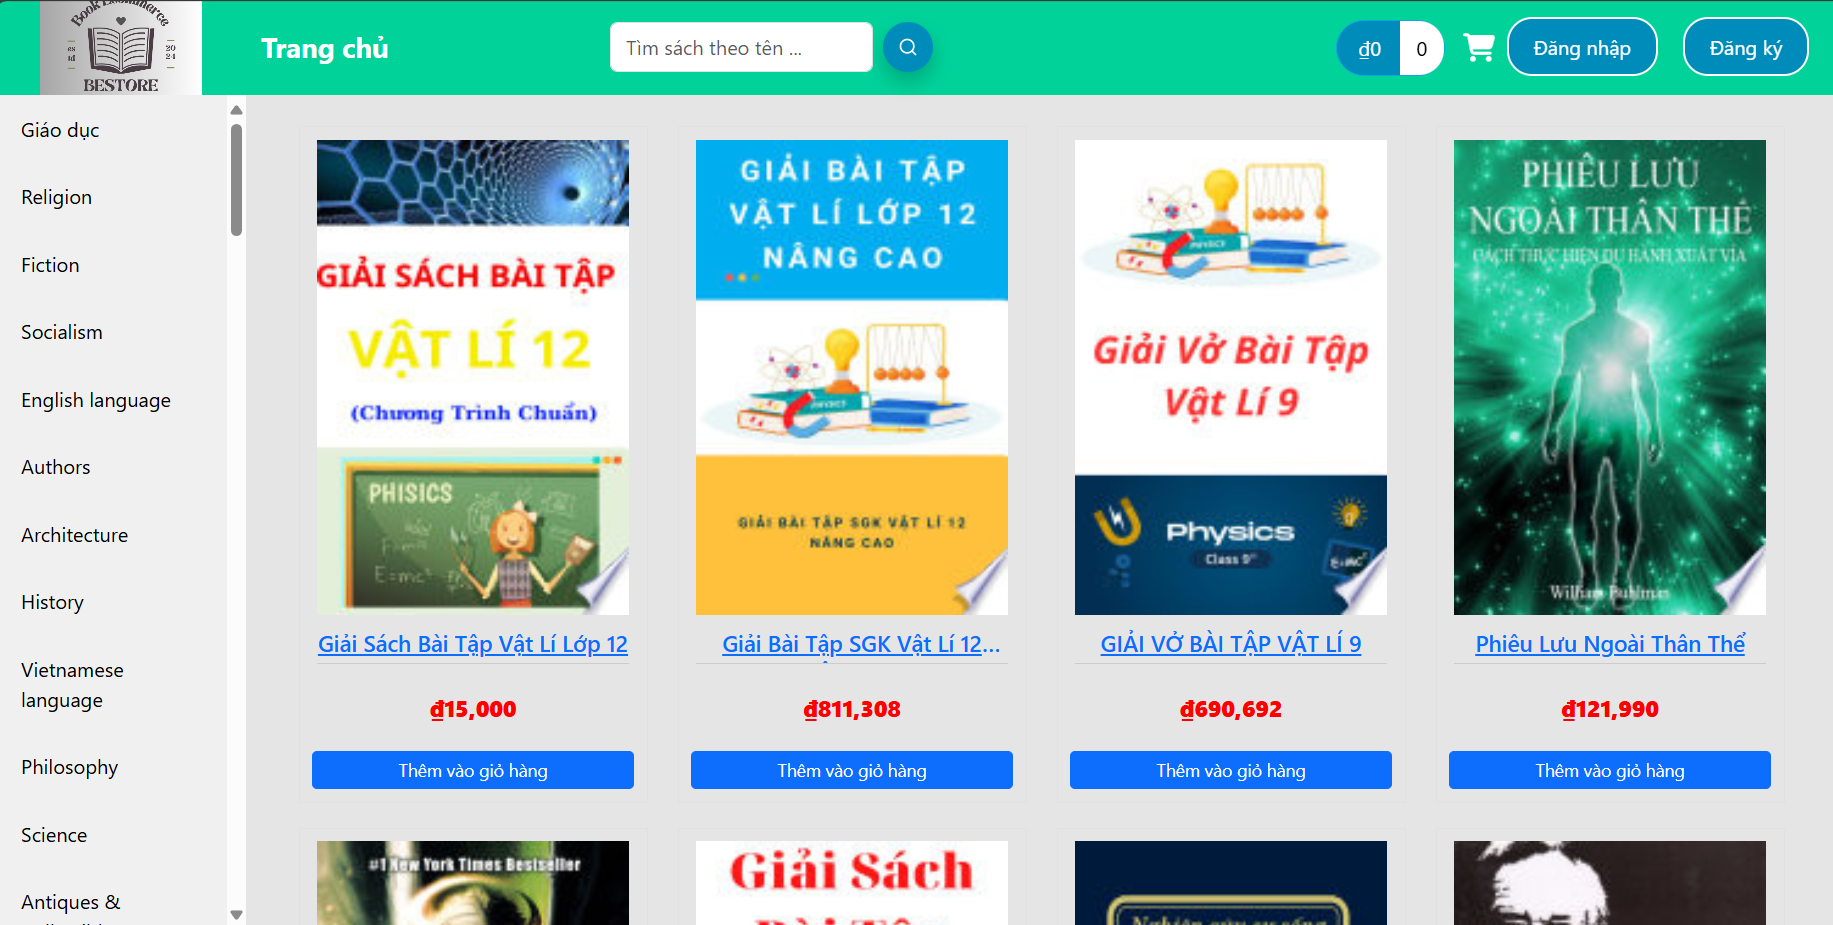
\includegraphics[width=1\linewidth]{Hinhve/màn hình trang chủ.png}
    \caption{Màn hình trang chủ}
    \label{fig:visual home}
\end{figure}

Màn hình trang chủ bao gồm có phần header chứa thanh tìm kiếm, giỏ hàng,nút đăng nhập, đăng ký. Phần Sidebar chứa danh mục của các loại sách và các quyển sách nằm ở phần còn lại.

\subsubsection{Màn hình tìm kiếm theo danh mục}
\begin{figure}[H]
    \centering
    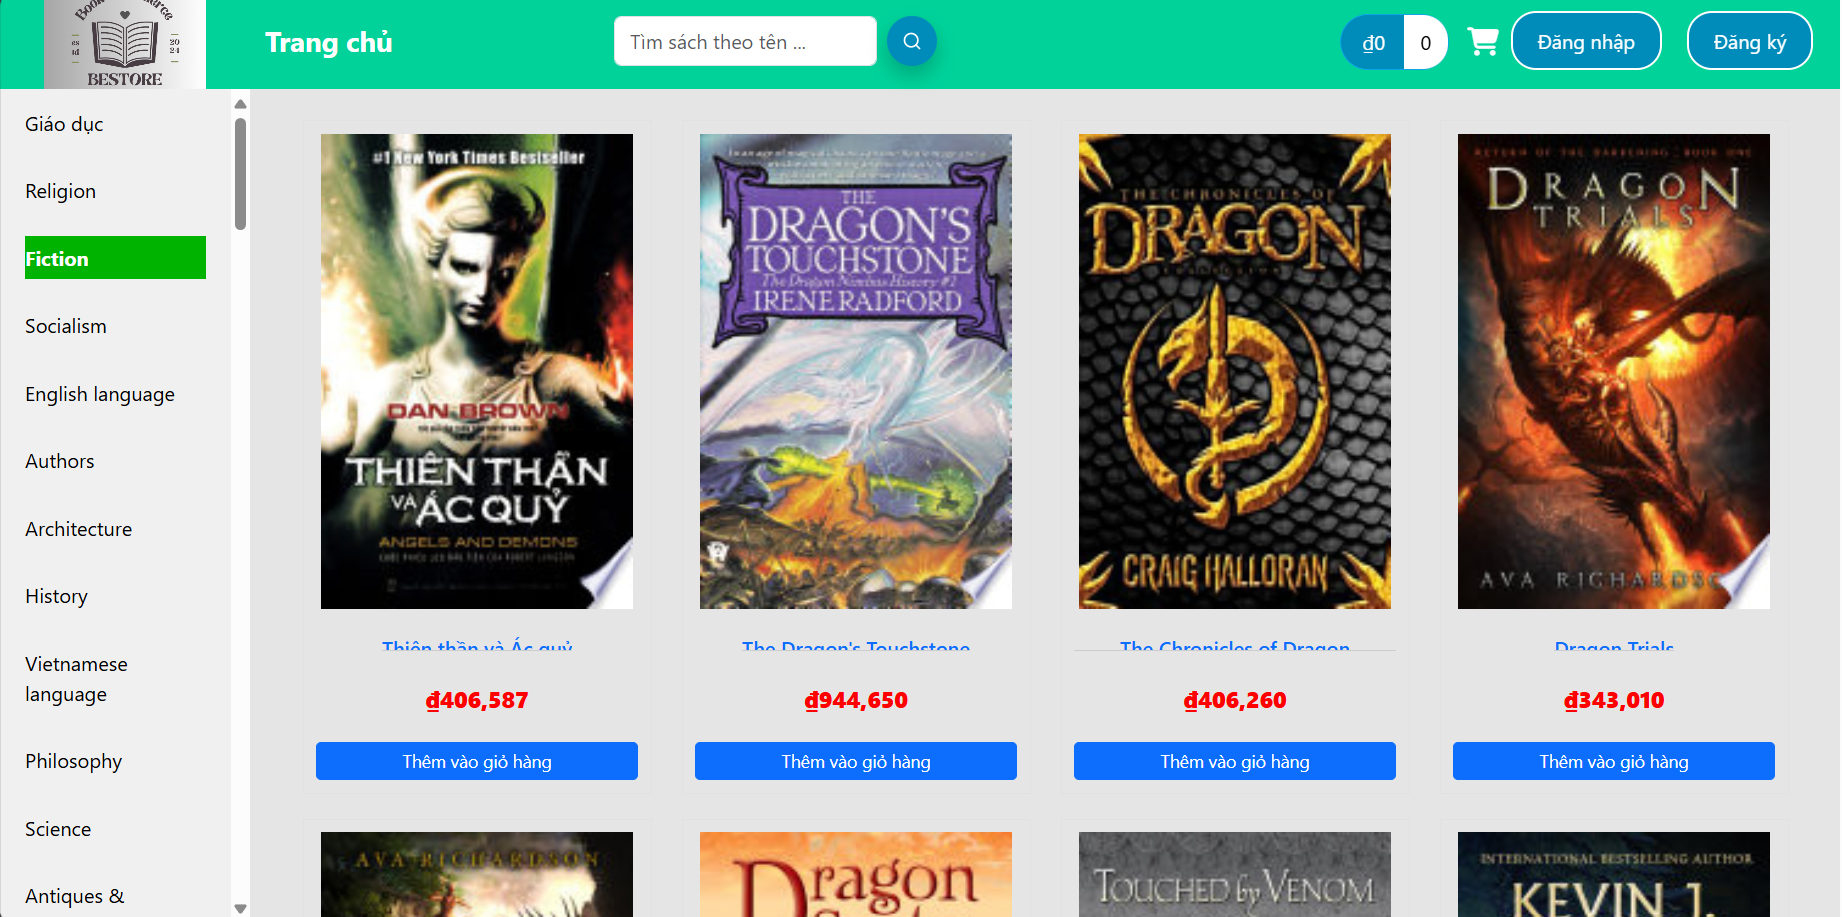
\includegraphics[width=1\linewidth]{Hinhve/tìm kiếm theo danh mục.png}
    \caption{Màn hình tìm kiếm theo danh mục}
    \label{fig:visual category}
\end{figure}

Màn hình tìm kiếm theo danh mục gần giống với màn hình trang chủ, khác ở những quyển sách thì là các sách có cùng danh mục.

\subsubsection{Màn hình giỏ hàng}
\begin{figure}[H]
    \centering
    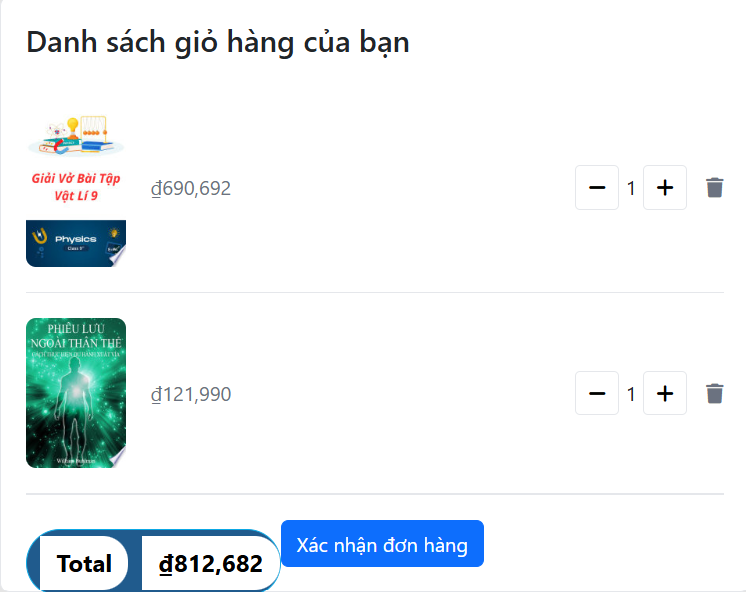
\includegraphics[width=1\linewidth]{Hinhve/giỏ hàng.png}
    \caption{Màn hình giỏ hàng}
    \label{fig:visual cart}
\end{figure}

Màn hình Màn hình giỏ hàng bao gồm danh sách các mặt hàng đã chọn, số lượng và giá thành và tổng tiền.

\subsubsection{Màn hình đăng ký}
\begin{figure}[H]
    \centering
    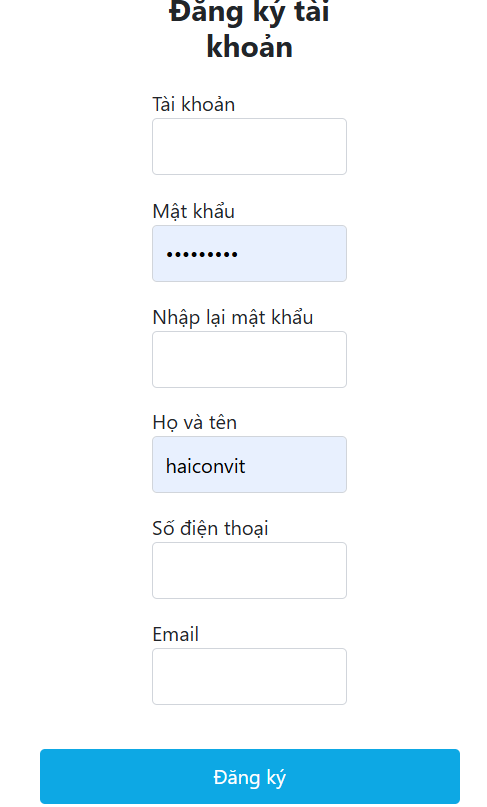
\includegraphics[width=0.8\linewidth]{Hinhve/đăng kí.png}
    \caption{Màn hình đăng ký}
    \label{fig:visual sign up}
\end{figure}

Màn hình đăng ký bao gồm các trường cần thiết để tạo tài khoản, cùng như nút đăng ký.

\subsubsection{Màn hình đăng nhập}
\begin{figure}[H]
    \centering
    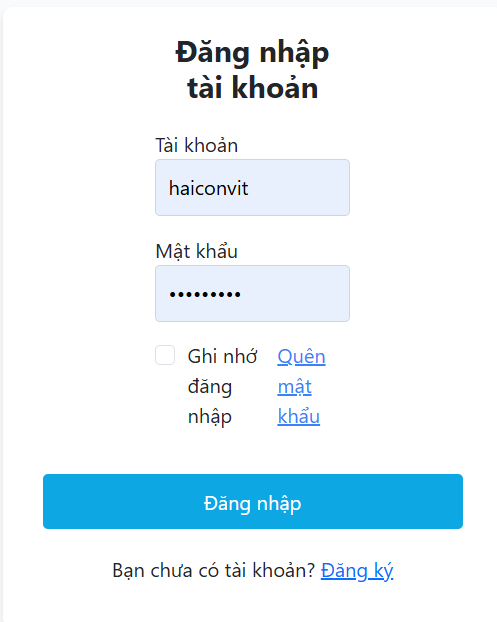
\includegraphics[width=1\textwidth]{Hinhve/đang nhập.png}
    \caption{Màn hình đăng nhập}
    \label{fig:visual sign in}
\end{figure}

Màn hình đăng nhập bao gồm trường tải khoản và mật khẩu và nút đăng nhập.

\subsubsection{Màn hình quản lý đơn hàng của admin}
\begin{figure}[H]
    \centering
    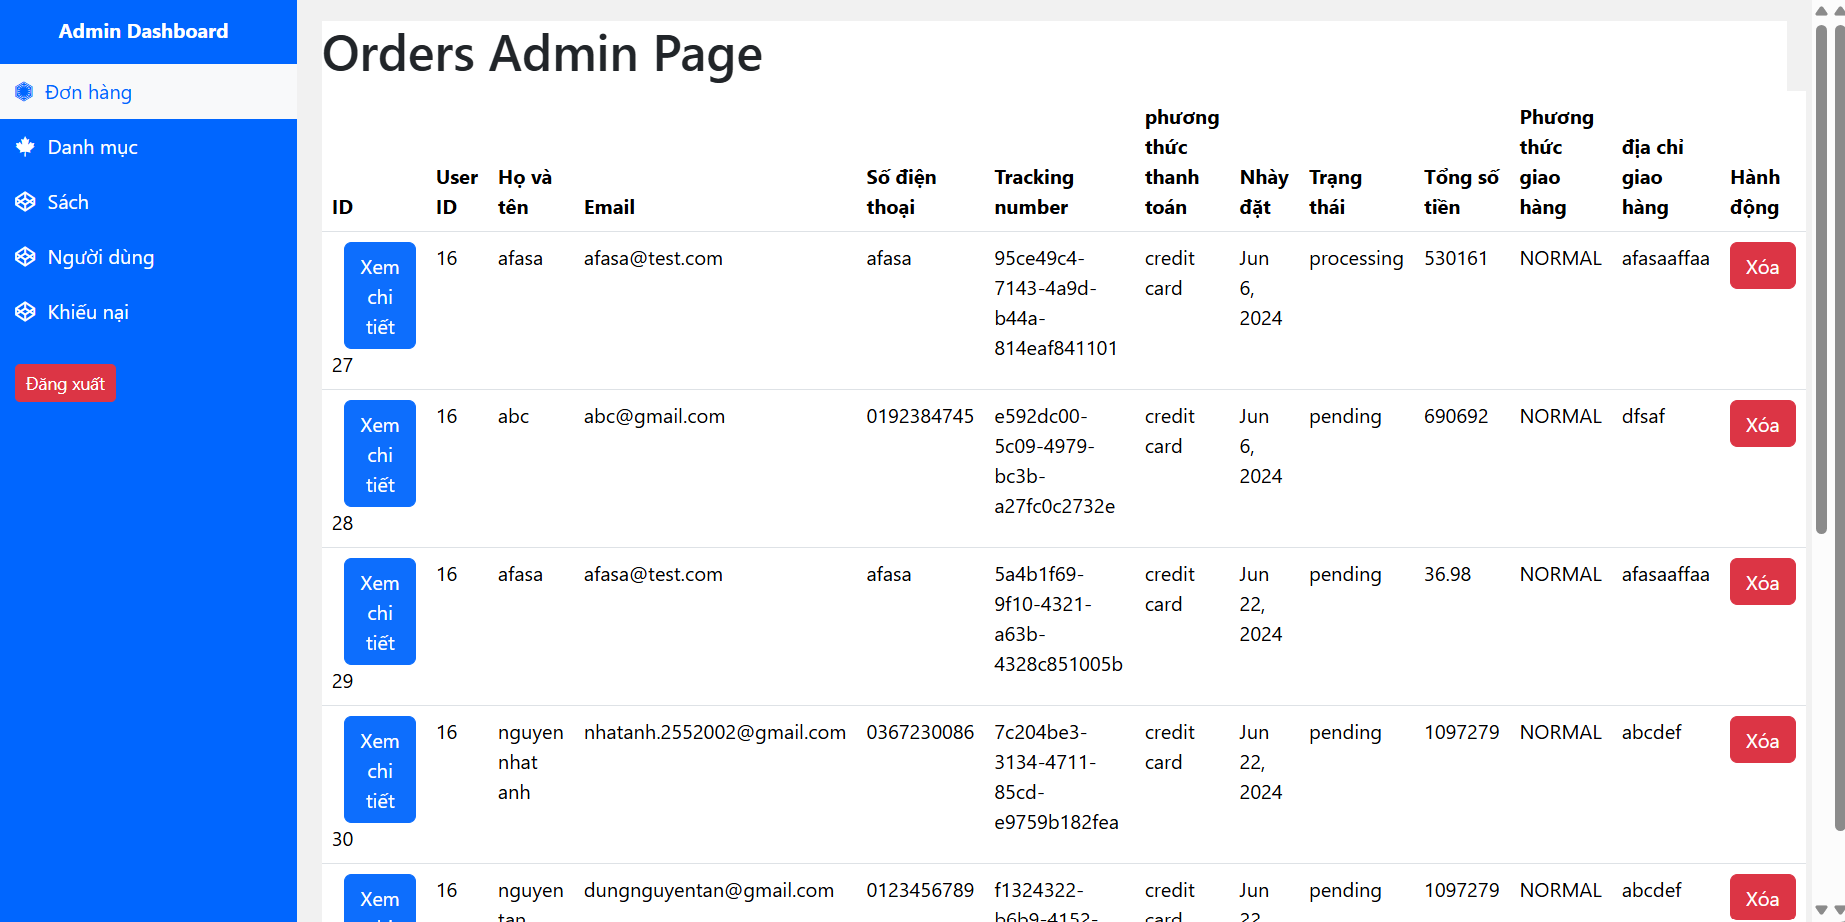
\includegraphics[width=1\linewidth]{Hinhve/order admin.png}
    \caption{Màn hình quản lý đơn hàng của admin}
    \label{fig:visual order admin}
\end{figure}

Màn hình quản lý đơn hàng của admin bao gồm phàn sidebar gồm có các phần mà admin quản lý như đơn hàng, sách, danh mục, khiếu nại. phàn còn lại thì hiển thị nội dung của những đơn hàng.

\subsubsection{Màn hình quản lý sách của admin}
\begin{figure}[H]
    \centering
    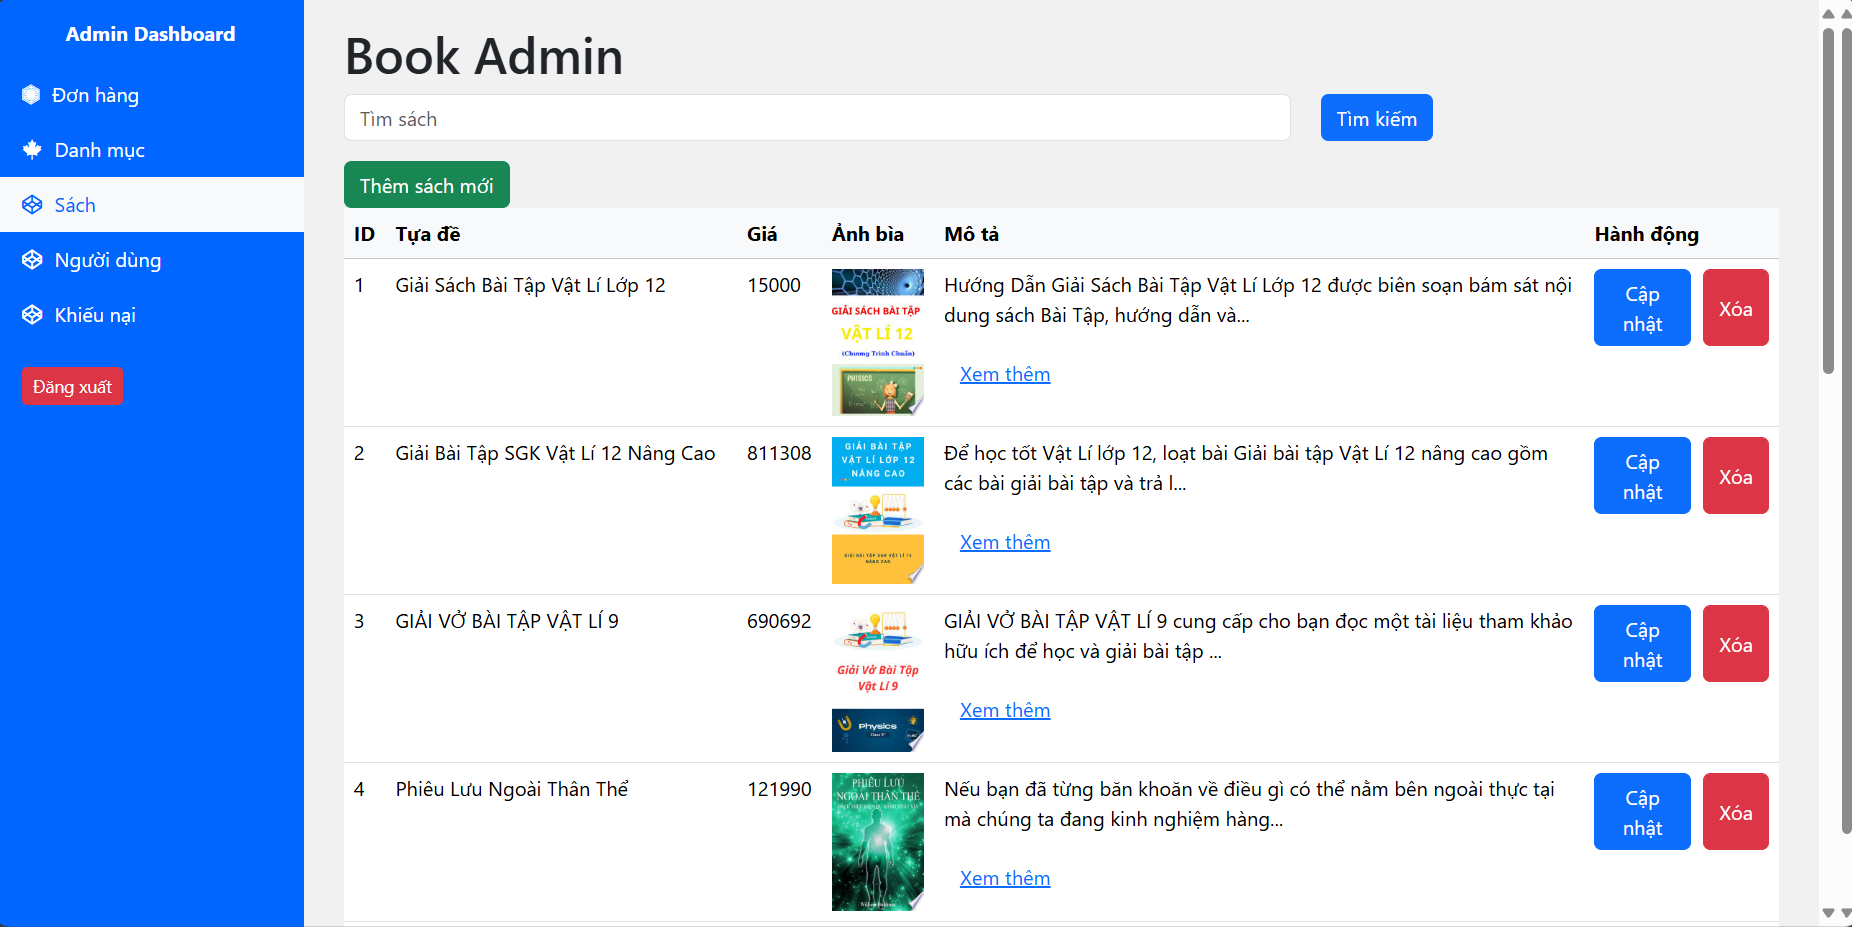
\includegraphics[width=1\linewidth]{Hinhve/book admin.png}
    \caption{Màn hình quản lý sách của admin}
    \label{fig:visual book admin}
\end{figure}

Màn hình quản lý sách của admin cũng giống như màn hình quản lý đơn hàng. Chỉ khác ở phần nội dung là bảng và thông tin về những quyển sách.
\section{Kiểm thử}
% Phần này có độ dài từ hai đến ba trang. Sinh viên thiết kế các trường hợp kiểm thử cho hai đến ba chức năng quan trọng nhất. Sinh viên cần chỉ rõ các kỹ thuật kiểm thử đã sử dụng. Chi tiết các trường hợp kiểm thử khác, nếu muốn trình bày, sinh viên đưa vào phần phụ lục.
% Sinh viên sau cùng tổng kết về số lượng các trường hợp kiểm thử và kết quả kiểm thử. Sinh viên cần phân tích lý do nếu kết quả kiểm thử không đạt.

Chức năng liên quan tới giỏ hàng và "Đặt hàng" là 2 trong nhiều chức năng quan trọng của hệ thống của tôi.
\subsubsection{Giỏ hàng}
\begin{NiceTabular}[width=1\linewidth]{X[1,l]X[2,l]X[5,l]X[3,l]}[hvlines]
\textbf{STT} & \textbf{Mô tả trường hợp thử nghiệm} & \textbf{Các bước kiểm tra} & \textbf{Kết quả} \\
1 & Thêm vào giỏ hàng & \begin{enumerate}
                        \item[(i)] Đăng nhập với tư cách người dùng
                        \item[(ii)] Chọn sách cần thêm vào giỏ hàng
                        \item[(iii)] Nhấn thêm vào giỏ hàng 
                        \end{enumerate}
& Quyển sách được thêm vào giỏ hàng tương ứng cới người dùng \\
2 & Chỉnh sửa số lượng của sách trong giỏ hàng
& \begin{enumerate}
    \item[(i)] Đăng nhập với tư cách người dùng
    \item[(ii)] Nhấn vào giỏ hàng để xem giỏ hàng của mình
    \item[(iii)] Nếu giỏ hàng trống, quay trở lại các trang danh mục hoặc
    trang chủ để chọn sách vào giỏ
    \item[(iv)] Nhấn các icon "+" và "-" để tăng giảm số lượng của sách trong giỏ hàng
\end{enumerate}
& Số lượng sách tăng giảm đúng như  ý muốn \\
\end{NiceTabular}

\begin{NiceTabular}[width=1\linewidth]{X[1,l]X[2,l]X[5,l]X[3,l]}[hvlines]
\textbf{STT} & \textbf{Mô tả trường hợp thử nghiệm} & \textbf{Các bước kiểm tra} & \textbf{Kết quả} \\
3 & Xóa sách trong giỏ hàng
& \begin{enumerate}
    \item[(i)] Đăng nhập với tư cách người dùng
    \item[(ii)] Nhấn vào giỏ hàng để xem giỏ hàng của mình
    \item[(iii)] Nếu giỏ hàng trống, quay trở lại các trang danh mục hoặc
    trang chủ để chọn sách vào giỏ
    \item[(iv)] Nhấn các icon thùng rác để loại bỏ quyển sách khỏi giỏ hàng
\end{enumerate}
 & Quyển sách được loại bỏ khỏi giỏ hàng  \\   
\end{NiceTabular}

\subsubsection{Đặt hàng}
\begin{NiceTabular}[width=1\linewidth]{X[1,l]X[2,l]X[5,l]X[3,l]}[hvlines]
\textbf{STT} & \textbf{Mô tả trường hợp thử nghiệm} & \textbf{Các bước kiểm tra} & \textbf{Kết quả} \\
1 & Đặt hàng và điền đủ các thông tin
& \begin{enumerate}
    \item[(i)] Đăng nhập với tư cách người dùng
    \item[(ii)] Nhấn vào giỏ hàng để xem giỏ hàng của mình
    \item[(iii)] Nếu giỏ hàng trống, quay trở lại các trang danh mục hoặc
    trang chủ để chọn sách vào giỏ
    \item[(iv)] Sau khi chọn lựa số lượng, nhấn "Xác nhận đặt hàng"
    \item[(v)] Ở màn hình đặt hàng, điền đầy đủ các thông tin về đơn hàng
    \item[(vi)] Nhấn đặt hàng
\end{enumerate}
 & Đơn hàng được tạo thành công  \\   
\end{NiceTabular}

\begin{NiceTabular}[width=1\linewidth]{X[1,l]X[2,l]X[5,l]X[3,l]}[hvlines]
\textbf{STT} & \textbf{Mô tả trường hợp thử nghiệm} & \textbf{Các bước kiểm tra} & \textbf{Kết quả} \\
2 & Đặt hàng và điền thiếu thông tin
& \begin{enumerate}
    \item[(i)] Đăng nhập với tư cách người dùng
    \item[(ii)] Nhấn vào giỏ hàng để xem giỏ hàng của mình
    \item[(iii)] Nếu giỏ hàng trống, quay trở lại các trang danh mục hoặc
    trang chủ để chọn sách vào giỏ
    \item[(iv)] Sau khi chọn lựa số lượng, nhấn "Xác nhận đặt hàng"
    \item[(v)] Ở màn hình đặt hàng, điền thiếu thông tin một số trường
    \item[(vi)] Nhấn đặt hàng
\end{enumerate}
 & Đơn hàng không được khởi tạo  \\   
\end{NiceTabular}

\subsubsection{Tổng kết về kiểm thử}
Trên đây là 5 trường hợp kiểm thử, với 4 trường hợp kiểm thử thành công và 1 trường hợp thất bại. Trường hợp thất bại do thiếu thông tin quan trọng nên không thể khởi tạo được đơn hàng.

\section{Triển khai}
% Sinh viên trình bày mô hình và/hoặc cách thức triển khai thử nghiệm/thực tế. Ứng dụng của sinh viên được triển khai trên server/thiết bị gì, cấu hình như thế nào. Kết quả triển khai thử nghiệm nếu có (số lượng người dùng, số lượng truy cập, thời gian phản hồi, phản hồi người dùng, khả năng chịu tải, các thống kê, v.v.)

Hệ thống bán sách trực tuyến của tôi sử dụng Spring Boot, AngularJS và MySQL được phát triển trên môi trường localhost, sử dụng máy tính cá nhân làm môi trường phát triển. Máy tính của tôi có cấu hình như sau:
\begin{enumerate}
    \item[(i)] \textbf{Hệ điều hành}: Window 11
    \item[(ii)] \textbf{Vị xử lý}: Ryzen 7 6800H
    \item[(iii)] \textbf{RAM} : 16GB
    \item[(iv)] \textbf{Ổ cứng}: SSD 512GB 
\end{enumerate}
Trước tiên tôi cài đặt Node.js phiển bản 20.9.0, MySQL phiển bản 8.0, Java phiển bản 17.0.10. Tôi cài đặt các IDE để viết mã cho phần BE và FE như InteliJ Idea Community Edition , VS Code.
Tổi tạo một dự án Spring Boot bằng cách khởi tạo trên \url{https://start.spring.io/} và tải file zip về máy. Sau đó tôi bắt đầu viết mã và thêm các package phụ trợ cho BE.
Về phần FE, tôi sủ dụng Node.js để cài đặt AngularJS phiển bản 17.3.5. Sau đó tôi khởi tạo dự án  Angular bằng câu lệnh "Ng new --no-Standalone " kèm với tên dự án FE. Sau đó tôi viết mã cho phần FE và cài đặt thêm các package để cấu hình cho dự án.
Về phần MySQL, tôi tạo 1 schema riêng cho dự án và xây dựng các bảng cần thiết. Dữ liệu về các cuốn sách được lấy từ Google Books Api. 
Trong quá trình cấu hình và phát triển mã nguồn, tôi chạy server Spring Boot  trên cổng 8080 và ứng dụng AngularJS trên cổng 4200. Tôi mở trình duyệt và truy cập vào http://localhost:4200 để kiểm tra giao diện người dùng và đảm bảo rằng các yêu cầu từ front-end được gửi đến back-end và phản hồi từ server được hiển thị chính xác. Khi gửi các yêu cầu từ giao diện người dùng, tôi kiểm tra xem server có xử lý đúng các yêu cầu và trả về kết quả mong muốn hay không. Tôi cũng dùng cả Postman để kiểm tra kết quả của các api ở bên phía BE trước khi ghép lại với FE.


\end{document}
